%%%%%%%%%%%%%%%%%%%%%%%%%%%%%%%%%%%%%%%%%%%%%%%%%%
\chapter{MATLAB}

%%%%%%%%%%%%%%%%%%%%%%%%%%%%%%%%%%%%%%%%%%%%%%%%%%


\section{El lenguaje y las bibliotecas}

Antes de entrar en materia es importante que sepamos qué diferencias
hay entre las sentencias de un lenguaje de programación y la
biblioteca de funciones.

Las sentencias son las palabras clave independientes. Esto significa
que si las eliminaremos del lenguaje no podríamos sustituirlas con
ninguna combinación del resto de sentencias del lenguaje. Esta
definición no es estricta; algunas palabras clave comunes se
consideran sentencias cuando se hace un uso muy frecuente de ellas.

El total de sentencias y de reglas de escritura son lo que forman el
lenguaje de programación descrito en un documento llamado
\emph{referencia\index{referencia}.}  Como Matlab es un programa
comercial no existe tal documento.

El resto de funciones y subrutinas son parte de la
\emph{biblioteca\index{biblioteca}}.  Son palabras clave que cumplen
una tarea y no pueden ser consideradas sentencias porque están
escritas con ellas. Algunas funciones de uso muy frecuente llegan a
ser parte del mismo lenguaje, el grupo que forman se llama
\emph{biblioteca estándar}\index{biblioteca estándar}.  El conjunto de
sentencias y biblioteca estándar se conoce como
\emph{especificaciones} y en el caso que el lenguaje tome vida propia,
es decir, sus especificaciones pasen a ser públicas; se llama
\emph{estándar}. Estos documentos existen para la mayoría de los
lenguajes de programación conocidos: C, C++, Ada, Fortran, Python...
Matlab no es uno de ellos.

Al ser un lenguaje sujeto a una herramienta Matlab es Matlab y punto;
sin embargo podemos aplicar estas definiciones estrictas para
acercarnos a él como lo haríamos con el resto de lenguajes. La
organización interna de Octave sigue este criterio. Se podría decir
que Octave es el conjunto de sentencias mas la biblioteca estándar y
que el resto de colecciones de funciones (y hay bastantes) son los
toolkits. La Compatibilidad entre los dos se sitúa sólo en las
sentencias aunque se extiende en gran manera con la biblioteca de
funciones. Por lo menos las funciones básicas son compatibles, casi
idénticas.

Matlab tiene muy pocas sentencias. Como lenguaje es muy sencillo
aunque cada versión incluye nuevas especificaciones. En los últimos
años se ha añadido la extensión para programación orientada a objetos
y el diseño de interfaces gráficas. Octave es ligeramente distinto en
su concepción; es más minimista y cuenta con muchas menos funciones
pero es más fácilmente extensible. Son las diferencias típicas entre
los productos libres y los comerciales.

Este capítulo es la referencia del lenguaje; en él veremos argumentos,
variables, operadores y sentencias que nos servirán para programar
funciones y scripts así como la arquitectura general del programa.  Es
con diferencia la parte más importante del libro y no se ha dividido
en varios capítulos para no romper el hilo conceptual.

\emph{Siempre que se hable exclusivamente de Matlab nos referiremos a
  las características comunes de Matlab y Octave. Cuando la palabra
  Matlab se utilice en una diferencia respecto a Octave nos estaremos
  refiriendo al programa comercial. Por sencillez no se ha
  diferenciado tipográficamente la palabra Matlab en los dos
  contextos.}


\section{Convenciones}

A partir de ahora escribiremos un comando escrito en la consola de la
siguiente manera:

\begin{verbatim}
>> %Esto es un comentario puesto en la consola de Matlab
\end{verbatim}
Escribiremos todas las palabras clave con letra de formato fijo como
esta función: \texttt{sin(x)}.

Veremos que la sintaxis de Matlab no es muy distinta de la de
cualquier otro lenguaje; las diferencias serán las de siempre, los
símbolos de continuación, los comentarios... Aunque sea un poco
temprano los listamos a continuación:

\begin{description}
\item [\texttt{'\_'}]Comillas simples. Sirven para introducir texto
  literal, todo lo que se encuentre en este entorno será tomado como
  texto y no como el nombre de una variable
\item [\texttt{{}``\_''}]Comillas dobles. Símbolo de carácter también
  soportado en Octave.
\item [\texttt{\%}]Porcentaje. Es el símbolo del comentario. Todo lo
  que está por detrás de este símbolo en una línea es ignorado por el
  intérprete.
\item [\texttt{\#}]Almohadilla. Símbolo del comentario sólo soportado
  por Octave. Es muy útil cuando se quieren añadir comentarios en la
  cabecera de una función sin que el parser\index{parser}%
  \footnote{Todos los lenguajes interpretados procesan el código con
    una herramienta llamada parser. El parser lee cada línea y
    distingue las palabras clave, las variables y los argumentos para
    que el intérprete pueda hacer su trabajo sin problemas.%
  } lo tome como parte de la ayuda.
\item [\texttt{...}]Tres puntos. Al añadir alguno de estos dos
  símbolos al final de una línea significa que se tomará la posterior
  como continuación
\item [\texttt{\textbackslash{}}]Barra invertida. El símbolo de
  continuación de C, C++ y Python también está soportado en Octave.
\item [\texttt{;}]Punto y coma. Símbolo de retorno de carro. Sirve
  para concatenar más de una sentencia en la misma línea y para
  inhibir la salida por consola del resultado.
\item [Importante:]El punto y coma al final de una sentencia explicita
  el retorno de carro e inhibe que salga el resultado por pantalla.
\end{description}

\subsection{Operaciones elementales con Matlab}

Las convenciones para las operaciones en Matlab son idénticas que en
cualquier otro lenguaje de programación o que en una calculadora
programable. El orden de asociación de las operaciones es también el
mismo. Primero se operan las funciones matemáticas elementales (senos,
cosenos, logaritmos...), las multiplicaciones y divisiones y luego
sumas y restas. Por ejemplo, para realizar la siguiente operación:
$$\frac{1}{\frac{2}{0.1^{1/2}}-\frac{0.4}{2^{1/3}}}$$
introduciremos enla consola:

\begin{verbatim}
>> 1/((2/0.1 ^(1/2))-(0.4/2 ^(1/3)))
\end{verbatim}

Evidentemente Matlab no distingue entre elementos numéricos y
variables, la ecuación:
$$\frac{a}{\frac{b}{c{}^{d}}-\frac{e}{g^{f}}}$$
\begin{verbatim}
>> a/(b/c^d-e/g^f)
\end{verbatim}

Los paréntesis sirven para variar el orden normal de las operaciones a
realizar.


\subsection{Algunas palabras clave y atajos de teclado.}

La consola es un entorno de trabajo más potente de lo que parece
gracias a una serie de atajos de teclado de gran utilidad. Uno de los
más potentes es la capacidad de auto-completar alguna palabra clave
con la tecla de tabular, tab completion en inglés. Por ejemplo, si nos
encontramos en el intérprete Octave y nos acordamos cómo se escribe
exactamente la función para trasponer una matriz podemos hacer lo
siguiente, escribimos sólo el inicio de la palabra y luego presionamos
la tecla de tabular:

\begin{verbatim}
>> tra<TAB>
trace      transpose  trapz
\end{verbatim}

Esta es una característica común de casi todas las consolas
existentes, ya sea una consola de UNIX o el Command Prompt de Windows.
La consola gráfica de Matlab es un poco más potente gracias a su
interfaz (figura \ref{cap:Tab-completion-en}):

%
\begin{figure}[h]
  \centering{}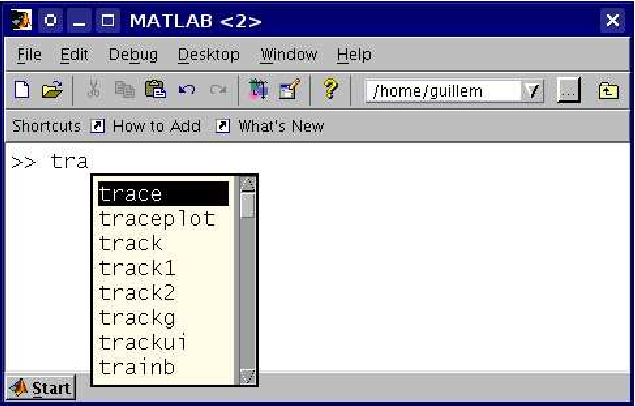
\includegraphics[width=8cm,
  keepaspectratio]{figuras/autocompletion}


  \caption{\label{cap:Tab-completion-en}Tab completion en Matlab}
\end{figure}


A continuación una lista de palabras clave y atajos de teclado que
pueden hacernos la vida mucho más fácil:

\begin{description}
\item [\texttt{exit}]Cierra el intérprete, equivalente a cerrar la
  ventana.
\item [\texttt{<CTRL>-c}]Corta la ejecución del comando actual (kill)
\item [$\uparrow$]Reescribe líneas anteriores. A medida que
  presionemos este carácter aparecerán en la línea actual todos los
  comandos escritos anteriormente. Una vez estemos viendo los comandos
  podemos movernos entre ellos mediante los cursores.
\item [\texttt{<CTRL>+<$\rightarrow$,$\leftarrow$>}]Hace avanzar o
  retroceder el cursor por palabras en vez de por caracteres.
\item [\texttt{clc}]Limpia la pantalla del intérprete de comandos
\end{description}

\section{La Ayuda(I)}

La manera más fácil de acceder a la ayuda tanto en Matlab como en
Octave es mediante la consola y el comando \texttt{help}\index{help}.
Cada comando y función lleva consigo la información necesaria para que
conozcamos su uso y sus funcionalidades%
\footnote{Más adelante aprenderemos cómo introducir esta información a
  cualquier función que escribamos%
}. Para acceder a la ayuda de una función teclearemos

\begin{verbatim}
>> help  {nombre de la función}
\end{verbatim}

Esto significa que debemos saber cómo se llama la función. Si
introducimos \texttt{help} sin ningún argumento nos aparecerá una
ayuda general desde donde podremos encontrar cualquiera de las
funciones disponibles.

Uno comando bastante útil cuando trabajamos desde una consola o por
red es \texttt{more}\index{more}. Si activamos el comando con
\texttt{more on} activaremos el paginador de modo que cuando el texto
que aparezca en pantalla se salga de la misma interrumpirá el texto
hasta que nosotros le pidamos que continúe. Esto evita el
comportamiento tan desagradable que tienen las ayudas especialmente
largas en las que siempre tenemos que utilizar la barra de
desplazamiento para ver el principio. Para salir del texto sin tener
que desplazarnos hasta el final pulsaremos la tecla \texttt{<Q>}.


\section{Tipos de archivos en Matlab}

Al igual que el intérprete es capaz de entender comandos mediante su
consola interactiva, también es capaz de leer archivos de código o
scripts. En el caso de Matlab los archivos asignados al intérprete
son los que terminan con la extensión \texttt{.m}. Pero para entender
cómo estos archivos interactúan con el intérprete es necesario 
que entendamos la arquitectura interna de Matlab.

Gran parte de la funcionalidad de Matlab se basa en su biblioteca de
funciones.  Una función en Matlab es equivalente a una función
matemática; es una tarea encapsulada que puede depender de una o
varias variables.  Matlab tiene una extensísima biblioteca de funciones, 
la mayoría de ellas son archivos con la extensión \texttt{.m} que
lee el intérprete.  Pero el intérprete no puede saber por ciencia infusa
dónde se encuentran dichas funciones.  Si en la consola introducimos:
\begin{verbatim}
>> sin(x)
\end{verbatim}
¿Cómo sabe Matlab dónde se encuentra la función seno?  La respuesta es
que Matlab ya sabe en qué directorios del sistema puede encontrar
archivos \texttt{.m} desde su instalación.

¿Significa esto que si creamos nuestras funciones debemos guardarlas
en estos directorios?  Ni mucho menos.  Matlab cuenta con un directorio
especial en el que también busca funciones; es el llamado \emph{directorio
de trabajo}.  Si estamos utilizando la interfaz gráfica de Matlab lo
seleccionaremos en la barra de herramientas.  Si en cambio accedemos 
a Matlab por consola o optamos por Octave el directorio de trabajo
será el directorio actual (en UNIX el contenido en la variable de
sistema PWD).  Cada vez que se invoque una función en Matlab buscará
en los directorios habituales y en el directorio de trabajo.

\subsection{Funciones(I)\label{sub:Funciones(I)}}

Una función\index{función} es una \emph{unidad de programa}, una tarea
independiente que puede o no depender de variables externas.  Las unidades
de programa típicas son las funciones, las subrutinas, las clases...
Matlab basa toda su potencia y su sencillez en el constante uso de
funciones.  La razón es bien sencilla; si Matlab es un programa para
cálculo numérico es normal que la unidad de programa esencial sea
la que tiene un significado más matemático

En Matlab se define una función del siguiente modo:\footnote{El comando
  \texttt{end} sólo es necesario en Octave cuando queremos acoplar
  funciones en los scripts o más de una función en un mismo archivo.
  En Matlab no es necesario porque cada función está asociada a un
  único archivo, el final del mismo hace de texttt{end}.}:

\begin{verbatim}
function [variables_de_salida]= nombre(variables_de_entrada)
  Comandos que terminamos asignando a las variables de salida
{end}
\end{verbatim}
 
Por ejemplo,si queremos implementar una función que sume dos escalares 
debemos hacer lo siguiente:

\begin{verbatim}
function [c]=suma(a,b)
  c=a+b;
\end{verbatim}

Y lo guardaremos en un archivo que se llame igual que la función; en
el caso del ejemplo será \texttt{suma.m}. Luego lo guardaremos en nuestro
directorio de trabajo.

El concepto de función va más allá pero esta descripción es suficiente
para entender su papel dentro de la arquitectura de Matlab.


\subsection{Scripts}

Los scripts hacen la función de un programa completo, su hilo de
sentencias tiene un principio y un final y no necesita actuar con
ninguna variable externa al código. La diferencia entre un
script\index{script} y un archivo de código fuente es que el script es
una transcripción literal de comandos de consola; se dice que es
\emph{secuencial}.  Esto no nos permite explotar las posibilidades de
los formatos libres ni utilizar secuencias de control tipo
\texttt{goto}%
\footnote{Mejor, porque este tipo de estructuras no son nada
  aconsejables.%
}. También tienen la extensión \texttt{.m} y se pueden ejecutar de
varios modos:

\begin{itemize}
\item Dentro del intérprete. Si hemos guardado el archivo en alguno de
  los directorios de búsqueda de funciones el intérprete ejecutará
  toda la secuencia de comandos introduciéndole el nombre del script
\end{itemize}
\begin{verbatim}
>> nombre_del_archivo
\end{verbatim}
\begin{itemize}
\item Fuera del intérprete. Dentro de una consola llamando el
  intérprete con el nombre de archivo como argumento. Por ejemplo, en
  una consola cualquiera:
\end{itemize}
\begin{verbatim}
$> matlab nombre_del_archivo
\end{verbatim}

Podemos llamar a funciones en nuestros scripts siempre que sea con
variables que hayamos inicializado antes de la llamada. El concepto es
el mismo, no es más que la transcripción de los comandos que se
introducirían en la consola.


\subsection{Nuestra primera función}

En esta primera función no usaremos ninguno de los elementos
característicos de la programación en Matlab. Estos son los que
encontramos en cualquier código de simulación: contadores, funciones
elementales, condicionales, casos... Empezaremos con el archivo
\texttt{aprsin.m}, que es la aproximación de orden 3 del desarrollo de
Taylor en 0 de la función seno. Para ello editamos el archivo nuevo de
nombre \texttt{aprsin.m} en el directorio que nos diga Matlab o Octave
según el caso y pondremos en ella lo siguiente:

\begin{verbatim}
function out=aprsin(x)
  out=x-x^3/6;
\end{verbatim}

Vemos que asignamos a la variable \texttt{out} las operaciones
que hacemos sobre la variable de entrada \texttt{x}. La idea es
mantener las características de una función matemática. Una vez la
hayamos guardado en el directorio de trabajo esta función puede ser llamada
por el intérprete de Matlab o por cualquier script.
Para probarlo nos vamos a la consola y tecleamos:

\begin{verbatim}
>> y=aprsin(1.3)
\end{verbatim}
que debe darnos como resultado:

\begin{verbatim}
y = 0.93383
\end{verbatim}
Aún es pronto para algunos conceptos, hay que aclarar un par de
cuestiones:

\begin{itemize}
\item Las variables \texttt{x} y \texttt{out} son de uso interno de la
  función.  Desde la consola o desde un script podemos usar las
  variables que queramos. Esta abstracción es común en todos los
  lenguajes de programación; la entenderemos cuando hablemos de la
  diferencia entre variable y argumento.
\item El punto y coma significa lo mismo que el retorno de carro.
  Tenemos que recordar siempre que la diferencia entre hacer un
  retorno de carro y poner el punto y coma es que en el segundo caso
  el programa no nos da ningún output. Llenaremos siempre las
  funciones de puntos y comas para no recibir resultados intermedios
  inútiles.
\end{itemize}

\subsection{Nuestro primer script}

Vamos a comparar nuestra aproximación de la función seno con la
función exacta y lo vamos a escribir en un guión. Para ello creamos el
archivo \texttt{comparar.m} y escribimos lo siguiente en él:

\begin{verbatim}
x=linspace(-pi,+pi,100);
for i=1:100
    y(i)=aprsin(x(i));
end
plot(x,[y;sin(x)])
\end{verbatim}
Para ejecutarlo vamos a la consola y tecleamos:

\begin{verbatim}
>> comparar
\end{verbatim}
E inmediatamente va a aparecer la figura \ref{cap:figura-ejemplo1}:


\begin{figure}[h]
  \centering{}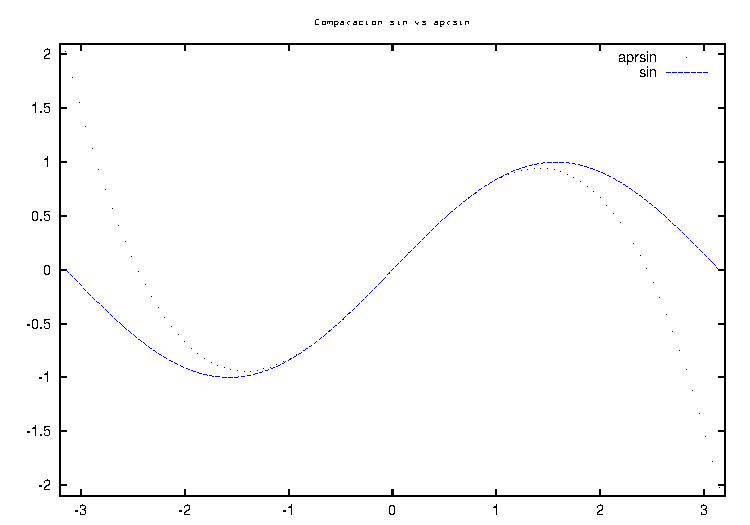
\includegraphics[%
  width=12cm,
  keepaspectratio]{figuras/figuraejemplo1}


  \caption{\label{cap:figura-ejemplo1}Comparación del desarrollo de
    Taylor}
\end{figure}


Aún es temprano para entender exactamente qué hace el script, lo
iremos viendo paso a paso; pero ha servido para ver cuál es la
relación entre funciones, los scripts y Matlab.


\subsection{Una gran diferencia entre Matlab y Octave}

\emph{Matlab no puede definir funciones directamente en el intérprete
o en un script.  Cualquier función debe ser un archivo independiente
por simple que esta sea}. Por ejemplo, si en Matlab escribimos:

\begin{verbatim}
>> function c=suma(a,b)
??? function c=suma(a,b)
    |
Error: Function definitions are not permitted at the prompt or in scripts.
\end{verbatim}
Recibimos un error.  En cambio Octave puede definir funciones tanto
en el intérprete como en un script, algo que dota a este intérprete
alternativo de algo más de versatilidad.

Éste es uno de los grandes puntos débiles de Matlab. Ignoro
el hecho por el que aún no lo soportan.

Lo que no se puede hacer ni en Matlab ni en Octave es acceder a varias
funciones distintas en un mismo archivo. No es muy difícil ver por
qué. El lenguaje Matlab, cuando llama a una función, busca por los
directorios algún archivo que se llame como la función, y luego busca
una sentencia ejecutable en él. Esto implica que cada archivo sólo
puede contener una cabecera%
\footnote{Puede contener más funciones pero sólo se puede llamar una.
  Esta es la función que tenga la cabecera en la primera linea cuyo
  nombre coincida con el nombre del archivo. Esta función puede llamar
  a otras funciones que se pueden encontrar en el mismo archivo, pero
  nunca podremos acceder desde fuera a las \emph{subfunciones} puesto
  que Matlab no tiene información para saber donde se encuentran%
}. Si pensamos un poco también vemos que en Octave se puede usar un
pequeño truco para cargar varias funciones sin necesitar una cabecera.
Simplemente creamos un script cuyo nombre no coincida con ninguna de
las funciones que contiene. Éste archivo lo empezamos con algo que no
sea la sentencia \texttt{function} y a continuación escribimos todas
las funciones que necesitemos. Luego, en el programa principal lo
llamamos con un:

\begin{verbatim}
>> source('header.m')
\end{verbatim}

\section{Argumento\index{Argumentos}}

El concepto preciso de argumento o valor es complejo pero a nosotros
nos bastará con saber que es cualquier elemento manipulable en un
código.  Los argumentos de un programa de simulación numérica son los
números, los índices, las matrices, las secuencias...

Tenemos que hacer el esfuerzo conceptual de separar el concepto de
argumento del de variable. Una variable es su contenedor, es lo que
les da nombre y sirve para manipularlos. Sucede lo mismo en cualquier
fórmula matemática; siempre se expresa mediante variables y toma
sentido cuando éstas contienen algún argumento.

Matlab tiene varios tipos de valores y variables; en consecuencia será
valida cualquier combinación entre ellos. Estos son los tipos de
argumentos soportados%
\footnote{Los físicos teóricos y los matemáticos encontrarán mucho más
  útil Python; lenguaje que probablemente desconozcan. La extensión
  numérica estándar de Python, numpy, soporta el tipo \emph{array}
  que es consistente con la definición de tensor. Esto permite operar
  con tensores de varias dimensiones de una forma mucho más natural.
  Es muy recomendable echarle un vistazo, la combinación de Python y
  la colección de bibliotecas SciPy es una mejor opción en el caso de
  aplicaciones más complejas en las que Matlab escale mal.%
}:


\subsection{Matrices\index{Matrices}}

Matlab no distingue entre escalares y matrices. Si se dice que Matlab
es un lenguaje de cálculo matricial es porque todos los números son en
el fondo matrices. El número $1$ puede ser escalar, vector y matriz a
la vez sin ningún problema:

\begin{verbatim}
>> a=1
a = 1
>> a(1)
ans = 1
>> a(1,1)
ans = 1
>> a(1,1,1)
ans = 1
\end{verbatim}
Tampoco distingue si sus elementos son enteros o reales, todos los
números tienen la misma precisión en coma flotante, que es doble
precisión siempre que no le indiquemos lo contrario. Las entradas

\begin{verbatim}
>> a=105
a = 105
>> a=1.05e+2
a = 105
>> a=1050e-1
a = 105
>> a=105.
a = 105
\end{verbatim}

son equivalentes. Estas son las dos características más importantes
del lenguaje.

Las matrices se estiran y encogen sin ninguna limitación ni en el
tamaño ni en las dimensiones. Si intentamos llenar el décimo elemento
de un vector \textbf{inexistente} con un 1.

\begin{verbatim}
>> foo(10)=1
\end{verbatim}
el programa lo va a hacer sin ningún problema

\begin{verbatim}
foo =   
  0  0  0  0  0  0  0  0  0  1
\end{verbatim}
y si ahora le pido

\begin{verbatim}
>> foo(11,4)=2
\end{verbatim}
obtengo

\begin{verbatim}
foo =   
  0  0  0  0  0  0  0  0  0  1   
  0  0  0  0  0  0  0  0  0  0   
  0  0  0  0  0  0  0  0  0  0   
  0  0  0  0  0  0  0  0  0  0   
  0  0  0  0  0  0  0  0  0  0   
  0  0  0  0  0  0  0  0  0  0   
  0  0  0  0  0  0  0  0  0  0   
  0  0  0  0  0  0  0  0  0  0   
  0  0  0  0  0  0  0  0  0  0   
  0  0  0  0  0  0  0  0  0  0   
  0  0  0  2  0  0  0  0  0  0
\end{verbatim}
Vemos que el comportamiento es un poco extraño. Si nosotros utilizamos
únicamente un índice obtenemos un vector fila, mientras que en una
matriz la notación es la usual, el primer elemento es el número de
fila y el segundo el número de columna. Esto nos obligará a trasponer
vectores más de una vez, sobretodo para resolver sistemas lineales de
ecuaciones%
\footnote{En Octave existe la variable
  \texttt{prefer\_column\_vectors}. Activando esta variable con
  \texttt{prefer\_column\_vectors=1} el vector por defecto será
  columna en vez de fila emulando el comportamiento de Fortran. Sirva
  esto para mostrar que Octave es totalmente configurable.%
}.

Esta característica facilita la tarea de escribir los algoritmos por
primera vez pero tiene grandes peligros \footnote{El principal peligro
  de la asignación dinámica de memoria es que nosotros no sabemos
  cuándo usamos demasiada. Es muy importante en códigos no usar más
  memoria en ningún momento que la RAM disponible, porque en el caso
  que 'pisemos' fuera de la RAM, el proceso empezará a escribir sobre
  el disco duro y el rendimiento puede bajar hasta en dos órdenes de
  magnitud. El problema es que en éste caso lo hacemos sin querer y
  además el programa no nos avisa.  Es bueno entonces tener algún
  monitor del sistema que nos diga cuánta memoria estamos usando en
  tiempo de ejecución y si estamos pisando fuera, es decir, escribimos
  en el espacio 'swap'. %
} e inconvenientes.

\begin{description}
\item [Importante:]Cualquier número es en realidad una matriz sin
  fronteras fijas.
\end{description}
Las matrices se ordenan en Matlab del mismo modo que en la realidad,
por filas y columnas. La notación para diferenciar si una serie de
números se encuentran en la misma fila o en la misma columna es el
siguiente:

\begin{itemize}
\item el espacio y la coma (,) separan elementos de una misma fila
\item el retorno de carro y el punto y coma (;) separan elementos de
  una misma columna
\end{itemize}
Por ejemplo, si queremos escribir el vector fila $\vec{e}=(1\ 2\ 3)$
lo haremos con:

\begin{verbatim}
>> e=[1,2,3]
e =
  1  2  3
>> e=[1 2 3]
e =
  1  2  3
\end{verbatim}
En cambio, para escribir el mismo vector pero en forma de columna:

\begin{verbatim}
>> f=[1;2;3]
f =
  1
  2
  3
>> f=[1
> 2
> 3]
f =
  1
  2
  3
\end{verbatim}
Esta es exactamente la misma notación que se sigue para introducir una
matriz entera. Lo intentamos con:
$$ \left(
  \begin{array}{ccc}
    1 & 2 & 3\\
    4 & 5 & 6\\
    7 & 8 & 9
  \end{array}\right)$$

\begin{verbatim}
>> m=[1,2,3;4,5,6;7,8,9]
m =
  1  2  3
  4  5  6
  7  8  9
\end{verbatim}
Aunque cualquier combinación de las anteriores sería perfectamente
válida, por ejemplo:

\begin{verbatim}
>> m=[1 2 3
> 4 5 6
> 7 8 9]
m =
  1  2  3
  4  5  6
  7  8  9
\end{verbatim}
La llamada simple a un elemento cualquiera de una matriz se hace
indicando su fila y su columna por ese orden. En el caso de la matriz
\texttt{m}:

\begin{verbatim}
>> m(2,1)
ans = 4
\end{verbatim}
Aprenderemos a crear matrices de más dimensiones en la sección
\ref{sub:Creaci=F3n-directa-de}.


\subsubsection{\label{argumentosmatriciales}Tipos de argumentos matriciales}

Cuando se habla del \emph{tipo} de un argumento no estamos hablando
sólo de si es una matriz, una cadena de caracteres, un número
complejo.  El concepto en el ámbito del cálculo numérico va mucho más
allá. Se llama \emph{tipo} a la representación que tiene un argumento
en la memoria del ordenador. Cuando almacenamos un número podemos
hacerlo en varias representaciones; coma flotante de simple precisión,
entero de 32 bits... Antes hemos hablado de la configuración por
defecto de Matlab que almacena todos los elementos de una matriz como
reales de doble precisión (64 bits o 8 bytes).

Todo lo dicho anteriormente para la representación interna de números
es válida sólo por defecto. En ningún momento afirmamos que el único
tipo de escalar posible es el real de doble precisión. Podemos definir
explícitamente números ,es decir, matrices; con tipos distintos al
real de doble precisión (DOUBLE).

Los tipos soportados por matlab son los mismos que C excepto por el
tipo \emph{long double} (real de 128 bits). Esta representación tiene
una limitación evidente; como la formulación de los argumentos en
Matlab es matricial sólo podremos tener matrices de un único tipo.  No
podremos construir matrices con elementos enteros y elementos reales a
la vez. Esta es una limitación común a todos los lenguajes de
programación y viene dado por la manera en la que cualquier programa
reserva (alocatea) memoria. Por ejemplo, si deseamos operar con
matrices de números enteros de 8 bits utilizaremos la función
\texttt{int8} del modo siguiente:

\begin{verbatim}
>> x=int8([1,2;109237401823056187365,83.0938])
x =
    1    2
  127   83
\end{verbatim}
Llama la atención el hecho de que el número 109237401823056187365 se
ha convertido en el 127. Esto es debido a que el mayor entero de 8
bits que podemos almacenar es precisamente 127. Si necesitamos una
aritmética de mayor precisión entera siempre podemos hacer lo
siguiente:

\begin{verbatim}
x=int64([1,2;109237401823056187365,83.0938])
x =
    1    2
  9223372036854775807   83
\end{verbatim}
Ni siquiera el mayor entero disponible es capaz de almacenar el número
anterior.
 
Podemos tener la necesidad de manipular la cantidad de memoria
dedicada a cada elemento de una matriz por dos motivos

\begin{enumerate}
\item Estamos definiendo matrices de gran tamaño y tenemos la
  necesidad de reducir la precisión de los argumentos reales; ya sea
  por la necesidad de reservar memoria o por requerimientos de
  velocidad de cálculo
\item Necesitamos operar con tipos de enteros, ya sean con signo o sin
  signo para realizar con ellos operaciones lógicas por bits o utilizar
  lógica entera.
\end{enumerate}
En Octave sólo es posible lo segundo porque el tipo de real es siempre
el de doble precisión. Hablaremos un poco más de los tipos de
argumentos escalares en la sección dedicada a rutinas de creación de
matrices.


\subsection{Secuencias\label{sub:Secuencias}}

Son parecidas a los vectores pero no lo son. Aparecen por todos los
elementos del lenguaje, en las submatrices, en los contadores en el
funcionamiento interno de muchas funciones... Siempre que necesitemos
contar algo aparecerán las secuencias porque \textbf{es el método
  propio Matlab para contar}. Si queremos una lista de números que nos
cuente del $1$ al $10$ hacerlo es tan fácil como:

\begin{verbatim}
>> secuencia=1:10
secuencia =
   1   2   3   4   5   6   7   8   9  10
\end{verbatim}
Si queremos manipular el contador para que no sea de $1$ en $1$
podemos introducir el salto entre dos números sucesivos:

\begin{verbatim}
>> secuencia=1:2:10
secuencia =
   1   3   5   7   9
\end{verbatim}


\subsubsection{Contadores no enteros.}

Las secuencias soportan intervalos distintos a los números enteros.
Podemos introducir la secuencia:

\begin{verbatim}
>> 0:0.5:4
ans =
 Columns 1 through 8:
  0.00000  0.50000  1.00000  1.50000  2.00000  2.50000  3.00000  3.50000
 Column 9:
  4.00000
\end{verbatim}

Si el intervalo que introducimos no ajusta exactamente al límite
superior parará de contar \emph{sin pasarse}.

\begin{verbatim}
>> 0:0.52:4
ans =
  0.00000  0.52000  1.04000  1.56000  2.08000  2.60000  3.12000  3.64000
\end{verbatim}
Evidentemente este tipo particular de contadores no son adecuados para
contar índices porque genera números no enteros. Su utilidad
se encuentra en la discretización de intervalos necesaria, por ejemplo,
en los ejes de coordenadas.


\subsection{Submatrices\index{Submatrices}}

Para asignar partes de matrices a variables o operar dentro de una
matriz con una parte de la misma es necesario asignarles una secuencia
de índices. Se puede decir que la submatriz se genera \emph{contando}
los índices de la primera Para entender mejor cómo funciona este tipo
de asignaciones mejor hacerlo mediante ejemplos. Iniciaremos una
sesión en Matlab creando una matriz de números aleatorios:

\begin{verbatim}
>> foo=rand(5,5)
 foo =
  0.808048  0.804808  0.871166  0.606412  0.867716
  0.114965  0.524531  0.210789  0.163542  0.639094
  0.476355  0.544236  0.254009  0.818164  0.091934
  0.736103  0.231876  0.115706  0.336303  0.478042
  0.807002  0.244172  0.507355  0.814160  0.792253
\end{verbatim}
Ahora crearemos una submatriz llamada \texttt{bar} que contendrá las
filas de la segunda a la quinta y columnas de la tercera a la quinta.

\begin{verbatim}
>> bar=foo(2:5,3:5)
 bar =
  0.210789  0.163542  0.639094
  0.254009  0.818164  0.091934
  0.115706  0.336303  0.478042
  0.507355  0.814160  0.792253
\end{verbatim}
Pero las secuencias tienen la capacidad de contar de modos distintos,
en el caso siguiente contaremos las filas de 2 en 2 como muestra el
siguiente ejemplo. En él crearemos una submatriz \texttt{qwe} que
sean, de la matriz \texttt{foo} las filas de la primera a la quinta de
2 en 2 (la primera, la tercera y la quinta) y las columnas de la
primera a la tercera.

\begin{verbatim}
>> qwe=foo(1:2:5,1:3)
 qwe =
  0.80805  0.80481  0.87117
  0.47635  0.54424  0.25401
  0.80700  0.24417  0.50735
\end{verbatim}
Si omitimos los elementos de la secuencia y dejamos sólo el símbolo
\texttt{:}, el resultado será que tomaremos todos los elementos de la
fila o de la columna.

Además de una secuencia los índices pueden introducirse mediante
vectores:

\begin{verbatim}
>> qwe=foo([1,2],[1,2])
\end{verbatim}

\subsection{Números Complejos \index{Números Complejos}}

En realidad deberían llamarse matrices cuyos elementos son números
complejos, pero se ha abreviado. Las reglas matriciales son
exactamente las mismas, lo único que cambia es el carácter individual
de cada elemento. La manera de introducir un número complejo como
argumento en una variable es el uso del número \texttt{i} que
multiplica a la parte imaginaria.

\begin{verbatim}
>> numcom=2+3i
\end{verbatim}

También podemos usar otros signos para expresar \texttt{$i$} como
\texttt{j}, \texttt{I} o \texttt{J}. Evidentemente también podemos
crear vectores, matrices y tensores de números complejos, y al buscar
un índice en ellos tendremos el número complejo completo.

Además del número \texttt{$i$} tenemos otros números relevantes
embebidos dentro de Matlab, como los números racionales $\pi$ como
\texttt{pi} o \texttt{e}.


\subsection{Cadenas de texto\index{texto}}

Podemos asignar a una variable una cadena de texto introduciéndola
entre comillas simples o dobles:

\begin{verbatim}
>> saludo='hola que tal';
\end{verbatim}
y si pedimos qué hay en la variable:

\begin{verbatim}
>> saludo
saludo = hola que tal
\end{verbatim}
En Octave también son válidas las comillas dobles:

\begin{verbatim}
>> saludo=''hola que tal''
saludo = hola que tal
\end{verbatim}
Matlab almacena las cadenas de texto como un vector de caracteres.
Esto significa que acepta todas las posibilidades de composición de
vectores, la diferencia es que operaremos con caracteres ASCII en vez
de con números reales. Para demostrarlo nada mejor que intentar
encadenar palabras en fila

\begin{verbatim}
>> ['me','gusta','el','furbo']
ans = megustaelfurbo
\end{verbatim}
o en columna

\begin{verbatim}
>> ['me';'gusta';'el';'furbo']
ans =
me
gusta
el
furbo
\end{verbatim}

\subsection{Argumentos lógicos\index{variables lógicas}}

Sólo tenemos dos variables lógicas que son \texttt{true} y
\texttt{false}.  Estos nombres son sólo interfaces, en realidad Matlab
toma \texttt{0} como falso y cualquier número distinto de cero como verdadero.


\section{Operadores\index{Operadores}}

Cuando operamos elementos en Matlab, como cuando lo hacemos en
cualquier lenguaje de programación, debemos tener en cuenta la
dicotomía entre variable y argumento. Es tan importante porque debemos
comprender perfectamente la sutileza de que los operadores no operan
variables sino argumentos, en el caso de Matlab, matrices.

La consecuencia directa es que todos los operadores de Matlab son
matriciales. En algunos casos, como la suma o la resta, los operadores
matriciales son equivalentes a lo escalares (\emph{elementwise}%
\footnote{\emph{Elementwise} significa literalmente en inglés elemento
  a elemento.%
} o elemento a elemento); en cambio la multiplicación y la potencia
generan resultados completamente distintos.

Por ejemplo, si tomamos dos matrices cualquiera:

\begin{verbatim}
>> A=[1 2 3;4 5 6;7 8 9];
>> B=[9 8 7;6 5 4;3 2 1];
\end{verbatim}

Su multiplicación directa va a dar como resultado precisamente la
multiplicación matricial:

\begin{verbatim}
>> A*B
ans =
   30   24   18
   84   69   54
  138  114   90
\end{verbatim}
¿Y si queremos una operación escalar? \textbf{Todos los operadores de
  Matlab pasan de matriciales a escalares añadiendo un punto justo
  antes del símbolo del operador}. En el caso de las matrices
anteriores:

\begin{verbatim}
>> A.*B
ans =
   9  16  21
  24  25  24
  21  16   9
\end{verbatim}
\textbf{La potencia es la operación que más errores provoca cuando se
  es principiante con el Matlab}. Cuando uno piensa en la operación de
la potencia nunca piensa en ella como una operación matricial; es muy
poco intuitivo. No pensamos que la operación:

\begin{verbatim}
>> A^2
\end{verbatim}
Sea equivalente a:

\begin{verbatim}
>> A*A;
\end{verbatim}

Operación que es matricialmente del todo lógica. Este comportamiento
provoca dos errores típicos.

\begin{enumerate}
\item El operador se negará a elevar a un exponente matrices que no
  sean cuadradas.
\item Cuando el exponente es fraccionario da resultados que
  aparentemente no tienen ninguna lógica
\end{enumerate}
Un ejemplo claro es lo que nos encontramos cuando elevamos la anterior
matriz a una burda aproximación del número $\pi$:

\begin{verbatim}
>> A^3.14
ans =
   691.22 -    0.43i   850.20 -    0.12i  1009.17 +    0.20i
  1567.33 -    0.05i  1925.90 -    0.01i  2284.47 +    0.02i
  2443.44 +    0.34i  3001.60 +    0.09i  3559.76 -    0.15i
\end{verbatim}
¿Números complejos?

El problema es que en Matlab cualquier argumento puede ser una matriz;
olvidarnos el punto antes de utilizar la potencia...

\begin{verbatim}
>> A.^3.14
ans =
    1.0000    8.8152   31.4891
   77.7085  156.5906  277.5843
  450.4098  685.0189  991.5657
\end{verbatim}
es uno de los errores más comunes. Por suerte los errores suelen ser
tan evidentes que la sangre raramente llega al río. El problema llega
cuando elevamos al cuadrado matrices cuadradas. Los resultados
obtenidos con el operador matricial y escalar son parecidos y del
mismo orden de magnitud con lo que pueden ser un gran escollo en el
proceso de depuración.


\subsection{Operadores aritméticos\index{Operadores aritméticos}}

\begin{description}
\item [\texttt{x+y}]Suma\index{Suma}. Si ambos operandos son matrices
  el número de filas y columnas debe ser el mismo. Si uno de los dos
  operandos es un escalar su valor es sumado a todos los elementos del
  otro
\item [\texttt{x-y}]Resta\index{Resta}. Las consideraciones sobre
  matrices son las mismas que con el operador suma.
\item [\texttt{x{*}y}]Multiplicación\index{Multiplicación} matricial.
  Si ambos elementos son matrices el número de filas y de columnas
  debe ser el mismo. Si uno de los dos operandos es un escalar su
  valor es multiplicado a todos los elementos del otro.
\item [\texttt{x.{*}y}]Multiplicación elemento a elemento. Si ambos
  operandos son matrices el número de filas y de columnas debe
  coincidir.
\item [\texttt{x/y}]{}``División de izquierda a derecha''. Esta
  operación es equivalente a:$$
  \left((y^{\top})^{-1}x^{\top}\right)^{\top}$$ con la diferencia que
  en este caso no se calcula la inversa. En el caso que la matriz $y$
  no sea cuadrada se da una solución con la condición de mínimo error%
  \footnote{Esto se hace calculando la pseudo inversa%
  }.
\item [\texttt{x./y}]División\index{División} de izquierda a derecha
  \emph{elementwise}.  Se divide cada elemento de la matriz $x$ por
  cada elemento de la matriz $y$.
\item [\texttt{x\textbackslash{}y}] División de derecha a izquierda.
  Esta operación es equivalente a:$$ x^{-1}y$$ y sirve para resolver
  sistemas de ecuaciones lineales. Como en la división anterior no se
  calcula efectivamente la inversa de la matriz, de modo que en el
  caso que no sea cuadrada seguirá dando un resultado.  Analizaremos
  este operador con mucha más profundidad en el apartado dedicado a
  álgebra lineal.
\item [\texttt{x.\textbackslash{}y}] División de derecha a izquierda
  \emph{elementwise}.
\item [\texttt{x\textasciicircum{}y}]
\item [\texttt{x{*}{*}y}]Potencia\index{Potencia}. Si ambos operadores
  son escalares el resultado es $x$ elevado a la potencia de $y$.  Si
  $x$ es un escalar y $y$ es una matriz cuadrada el resultado se
  calcula a partir de un desarrollo de autovalores. Si $x$ es una
  matriz cuadrada e $y$ es un entero el resultado es la multiplicación
  de $x$ por ella misma $y$ veces y si $y$ es un real se calcula el
  resultado por un desarrollo de autovalores. Cuando tanto $x$ como
  $y$ son matrices el resultado es error. La notación \texttt{{*}{*}}
  sólo se puede usar en Octave.
\item [\texttt{x.\textasciicircum{}y}]~
\item [\texttt{x.{*}{*}y}]Potencia \emph{elementwise}. Si los dos
  operandos son matrices deben ser del mismo tamaño. La notación
  \texttt{.{*}{*}} sólo se puede usar en Octave
\item [\texttt{-x}]Negación\index{Negación}
\item [\texttt{x'}]Traspuesta\index{Traspuesta} compleja conjugada. Si
  la matriz $x$ está compuesta por números reales el resultado es
  exactamente el mismo que para la traspuesta. Si hay algún argumento
  complejo el operador es equivalente a hacer \texttt{conj(x.')}.
\item [\texttt{x.'}]Traspuesta \footnote{Esta es una buena manera de
    perder un día de trabajo tontamente. Es de estos errores que hacen
    que te rompas la cabeza intentando entender qué es lo que funciona
    mal.

    Cuando se trabaja en el espacio de Fourier es muy normal que todos
    los coeficientes sean complejos. Además, si los datos que originan
    los coeficientes son reales la matriz que forman es hermitiana que
    es como la extensión de la matriz simétrica para números
    complejos.

    Probando un algoritmo de de resolución de la ecuación de Poisson
    en el plano espectral me puse a probar qué era lo que calculaba la
    transformada rápida de Fourier (se verá en los temas posteriores)
    bidimensional y si era equivalente con una combinación de
    transformadas unidimensionales.  En teoría el algoritmo de
    transformada rápida de Fourier en un plano es transformar por
    columnas y luego hacerlo por filas. Como la función transformada
    rápida de Fourier en Matlab es \texttt{fft} la operación sería


    \texttt{>{}>fft(fft(a)')'} Con esto se hace la operación por
    columnas, se traspone, se hace la operación por filas y se vuelve
    a trasponer para devolver la matriz a su estado inicial. Esta
    operación debería ser equivalente a:

    \texttt{>{}>fft2(a)} Cual fue mi sorpresa cuando descubrí que los
    coeficientes que daba como resultado eran distintos. No es que el
    resultado tenga que ser equivalente, es que tiene que ser
    exactamente el mismo.  Después de \textbf{ocho} horas de revisar
    una y otra vez los resultados me dí cuenta que el operador
    \texttt{'} no es la traspuesta sino la traspuesta compleja
    conjugada y que en este caso no son equivalentes porque el
    resultado no es una matriz hermitiana hasta que se ha terminado la
    transformada. Entonces la operación sería:

    \texttt{>{}>fft(fft(a).').'}

    Esta tontería bien puede haceros perder un día, como a mi, o un
    par de ellos por culpa de resultados que parecen válidos. Mucho
    cuidado.

    A título de opinión personal creo que este es un gran fallo en la
    sintaxis general de matlab. Hay más, incluso peores. Esto debería
    corregirse como en otros lenguajes donde los operadores tienen su
    forma abreviada (\texttt{*}) y una forma equivalente como
    función}.  Nótese que el uso de la notación usual
  \emph{elementwise} no tiene el mismo sentido.
\end{description}

\subsection{Operadores de comparación\index{operadores de
    comparación}}

\begin{description}
\item [\texttt{x<y}]Verdadero si $x$ es menor que $y$.
\item [\texttt{x<=y}]Verdadero si $x$ es menor o igual que $y$.
\item [\texttt{x==y}]Verdadero si $x$ es igual que $y$.
\item [\texttt{x>=y}]Verdadero si $x$ es mayor o igual que $y$.
\item [\texttt{x>y}]Verdadero si $x$ es mayor que $y$.
\item [\texttt{x!=y}]~
\item [\texttt{x\textasciitilde{}=y}]Verdadero si $x$ es distinto que
  $y$. En Octave son válidos ambos signos mientras que Matlab sólo
  soporta el segundo.
\end{description}

\subsection{Operadores lógicos\index{operadores lógicos}}

Hay dos tipos de operaciones lógicos, los que interactúan con matrices
y los que lo hacen con expresiones lógicas como las que nos
encontramos en las estructuras \texttt{if} y \texttt{while}. Los del
primer tipo son \texttt{\&} para {}``y\index{y}'', \texttt{|} para
{}``o\index{o}'' y \texttt{!} para {}``no\index{no}''. Si decimos que
operan con matrices es porque aplicados a matrices de condiciones
lógicas devuelven una matriz del mismo tamaño, por ejemplo:

\begin{verbatim}
>> [1,2;0,1]&[0,1;0,1]
ans =
  0  1
  0  1
>> ![0,1;2,0]
ans =
  1  0
  0  1
\end{verbatim}
La expresión entera para condiciones lógicas es \texttt{0} para
{}``falso'' y distinto de \texttt{0} para {}``verdadero'', es decir,
lógica binaria usual.

Para componer expresiones lógicas se usan los símbolos \texttt{\&\&}
para {}``y'' y \texttt{||} para {}``o''. La diferencia entre estos y
los anteriores es que el resultado siempre será booleano. Si se aplica
a una matriz colapsará sus elementos con la función \texttt{all} para
llegar a una expresión única. Como ya hemos dicho antes su aplicación
principal se encuentra en las estructuras de control de ejecución como
\texttt{if} y \texttt{while}.

En los capítulos posteriores veremos varias aplicaciones de estos
operadores.


\subsection{Operadores de comparación por bits en enteros}

Matlab es también capaz de comparar y manipular los bits en enteros.
Para eso dispone de las funciones siguientes:
\begin{verbatim}
>> bit<TAB>
bitand    bitmax    bitset    bitxor
bitcmp    bitget    bitor     bitshift
>> a=5; %Un numero entero
>> dec2bin(a) %Que tiene esta representacion decimal
ans = 101
>> a=bitset(a,1,0) %Reset del primer bit
a = 4
>> a=bitset(a,6,1) %Set del sexto bit
a = 36
>> dec2bin(a)
ans = 100100
>> b=bitset(1,6) % Una forma alternativa de set
b = 33
>> dec2bin(b)
ans = 100001
>> bitand(a,b) % y logico
ans = 32
>> dec2bin(bitand(a,b)) % En bits...
ans = 100000
>> bitor(a,b) % o logico
ans = 37
>> dec2bin(bitor(a,b)) % En bits...
ans = 100101
>> bitxor(a,b) % o exclusivo logico
ans = 5
>> dec2bin(bitxor(a,b)) % En bits...
ans = 101
\end{verbatim}

\section{Variables\index{Variables}}

Debemos pensar en ellas como cajas que ocupan memoria,
independientemente de lo que lleven dentro. Debe abstraerse la
variable del argumento que contenga, en el fondo no es más que un
nombre.

Por el hecho de ser un lenguaje de scripting las variables no deben
declararse. Esto hace que programar sea mucho más sencillo, se haga
con menos errores y en menos tiempo a costa de un mayor tiempo de
ejecución. Esto también significa que la cantidad de memoria asignada
a una variable es dinámica, podemos ampliar una matriz %
\footnote{Ampliar una matriz es exactamente equivalente que asignar
  más memoria a una variable. En Fortran sería dealocatear una
  variable, ampliarla y alocatearla otra vez.%
} sin ningún problema con el simple hecho de llenar un elemento que no
exista.

Aquello que nosotros asignamos a una variable se llamará argumento%
\footnote{El concepto de argumento en programación es mucho más extenso, pero
creo que es conveniente usarlo de este modo.%
}. A cada variable le asignaremos uno o varios argumentos, de modo
que la variable no es más que un nombre por el que llamamos su contenido.

Las variables pueden ser cualquier secuencia de letras, no hay
limitación en su número, sólo que deben empezar con un carácter tipo
letra o con \_ . Se distingue entre mayúsculas y minúsculas. Los
nombres siguientes serían válidos:

\begin{verbatim}
x
x15
__hola_que_tal__
fjalsbdgaoqiwbodj
\end{verbatim}
El nombre de una variable es una función en sí misma, llamada sin
argumentos sacará por pantalla el valor de la variable. Algunas
variables tienen un valor por defecto como \texttt{pi} o \texttt{ans}.
Algunas de estas variables son parte de la configuración interna del
programa así que es importante conocerlas para no tener sorpresas
desagradables.


\subsection{Acceso a las variables:}

Si nos dicen que una variable es local por defecto probablemente no
entendamos nada. Saber si una variable es accesible o no por una
función no es una tarea sencilla y depende de cómo se hayan declarado
las variables. El esquema normal es el de la figura
\ref{cap:Comportamiento-normal-de}.  Supongamos que somos una variable
en el programa principal y en un instante de la ejecución somos el
argumento de una función. No nos sucede absolutamente nada. Otra
variable va a tomar nuestro valor en la cabecera de la función y su
resultado se va a volcar en el programa principal. A no ser que el
resultado se nos asigne, cambiando nuestro valor, seguirá sin
sucedernos nada. En cambio las variables locales para la función son
eliminadas de la memoria cuando termina su ejecución.

%
\begin{figure}[h]
  \centering{}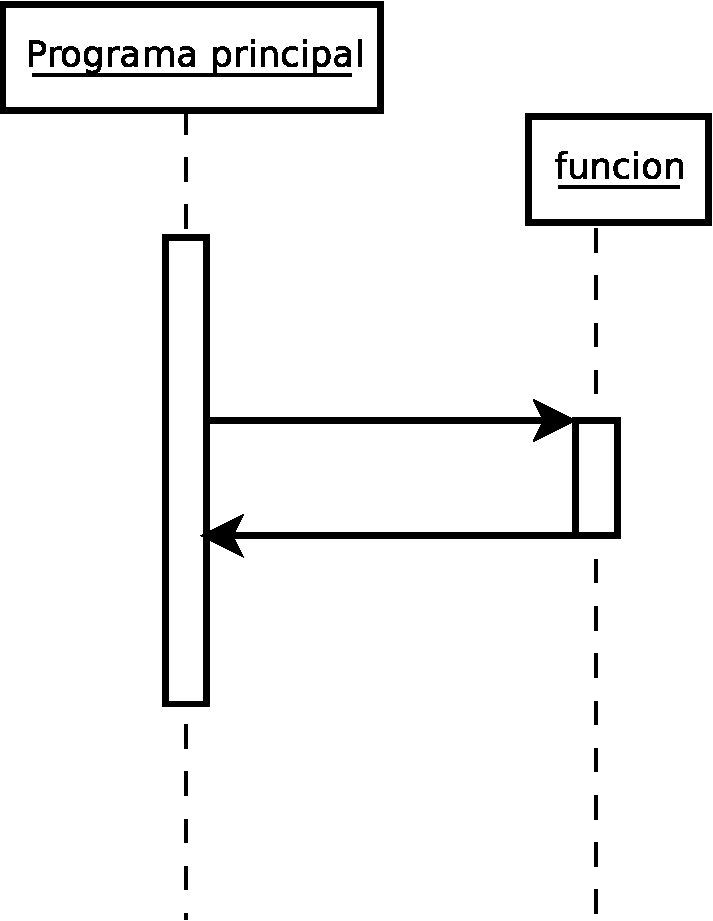
\includegraphics[%
  width=5cm,
  keepaspectratio]{figuras/Diagram1}


  \caption{\label{cap:Comportamiento-normal-de}Comportamiento normal
    de una variable llamada por una función}
\end{figure}


Si le damos a una variable el atributo de \emph{global} con la palabra
clave \texttt{global\index{global}} entonces esta variable podrá ser
vista por cualquier unidad de código sin necesidad de llamarla en su
cabecera. A estas variables no les importa si están en el programa
principal o en una función, su contexto es toda la ejecución; pueden
saltar a cualquier hilo como en el esquema de la figura
\ref{cap:Comprtamiento-de-una}:

%
\begin{figure}[h]
  \centering{}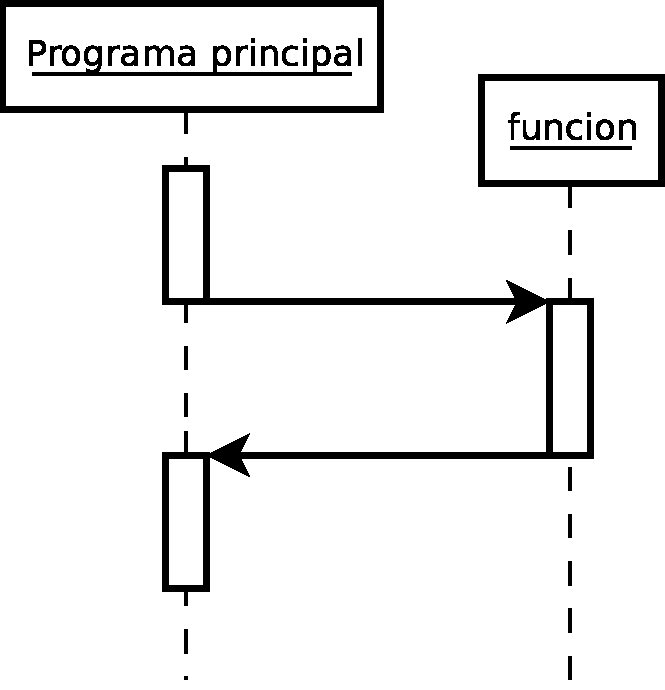
\includegraphics[%
  width=5cm,
  keepaspectratio]{figuras/Diagram2}


  \caption{\label{cap:Comprtamiento-de-una}Comportamiento de una
    variable global definida en el programa principal}
\end{figure}


Al estar definida como una variable global no sólo puede ser vista por
la función; si además la función cambia su valor también cambiará en
el programa principal. Un ejemplo de ello es el código siguiente:

\begin{verbatim}
>> global x=2
>> x
x = 2
>> function f()
global x
x=3
end
>> f()
x = 3
\end{verbatim}
Como se ve debemos tener cuidado con los nombres de las variables
globales, no es difícil estropear el código llamando una variable
global en una función sin querer%
\footnote{El uso de las variables globales es una de las pocas
  discusiones de estilo abiertas. En otros lenguajes de programación,
  sobre todo los que permiten la programación orientada a objetos, no
  es necesario utilizar este tipo de variables. Es una discusión entre
  dos escuelas.  Los que estamos más acostumbrados a una programación
  modular (Fortran) nos sentimos más cómodos controlando el hilo de
  ejecución con variables globales. En cambio, la escuela procedente
  de C++ y de Java prefieren crear métodos mucho más ricos en los que
  las funciones son en realidad métodos de un objeto que puede haber
  sido inicializado previamente.

  Creo que para un principiante el uso de variables globales es un
  buen ejercicio mental para aprender que hay distintos niveles de
  ejecución en la programación modular sin entrar en conceptos que
  muchos usan pero sólo unos pocos entienden.%
}.

Un tercer atributo es el de \texttt{persistent}\index{persistent}.
Cuando dentro de una función indicamos que una variable es
\texttt{persistent} estamos imponiendo que esta variable se guarde en
memoria para la siguiente vez que se llame la función en vez de
hacerla desaparecer, como es normal. El diagrama conceptual es el de
la figura \ref{cap:Propiedades-de-una}.

%
\begin{figure}[h]
  \centering{}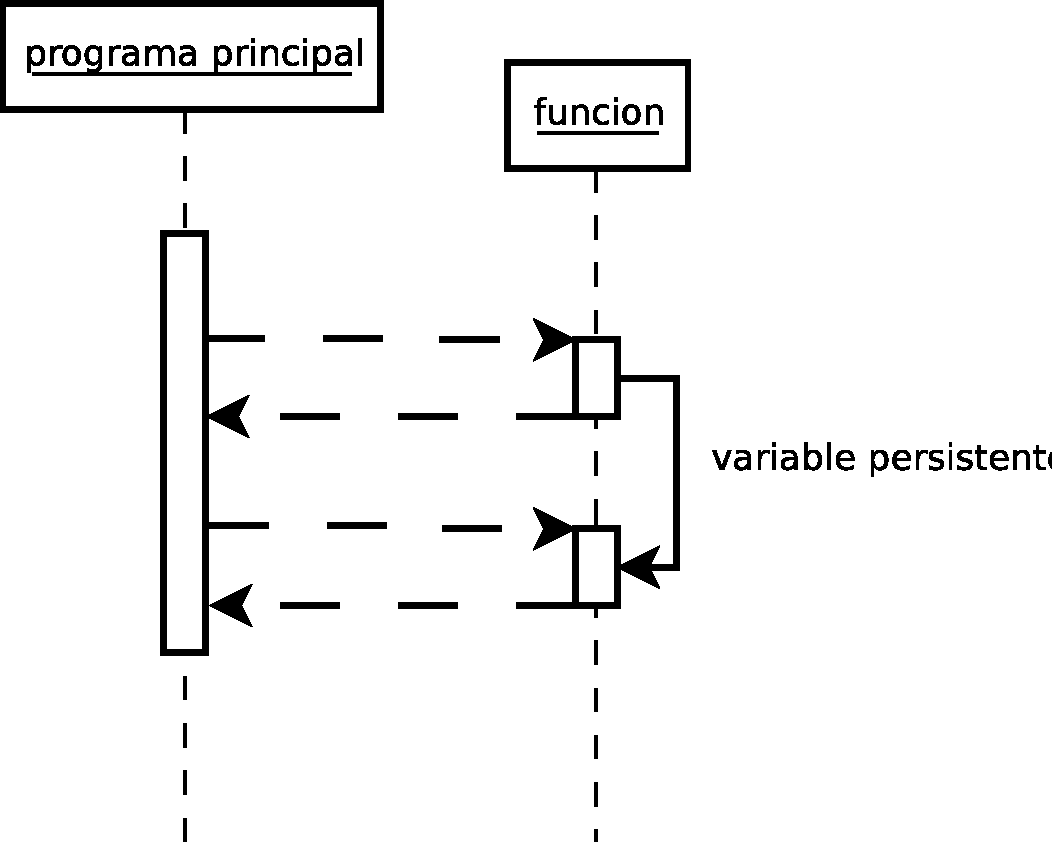
\includegraphics[%
  width=7.5cm]{figuras/Diagram3}


  \caption{\label{cap:Propiedades-de-una}Propiedades de una variable
    persistente.}
\end{figure}


No tiene ningún sentido definir una variable como \texttt{persistent}
en el programa principal porque las variables locales para el hilo
principal no se destruyen hasta que termina la ejecución.


\subsection{Funciones dedicadas a variables}

Tenemos varias funciones íntimamente relacionadas con el concepto de
variable, algunas de ellas son:

\begin{itemize}
\item \texttt{is\_global} que devuelve un $1$ en el caso que la
  variable efectivamente lo sea
\item \texttt{clear\index{clear}} que borra el contenido de una o
  varias variables, funciones o variables globales dependiendo del
  parámetro que le pasemos
\item \texttt{who\index{who}} que da una lista de las variables que en
  aquél mismo momento estén ocupadas por algún argumento. También
  acepta parámetros para variar su comportamiento.
\item \texttt{whos\index{whos}} , lo mismo que \texttt{who} pero nos
  da más información.
\end{itemize}
\begin{description}
\item [Importante:]Es necesario entender el concepto de variable local
  y global para comunicar funciones y scripts de una manera eficiente
\end{description}

\subsection{Contenedores\index{Contenedores}}

La limitación las matrices es que sólo pueden contener
elementos de un mismo tipo.  Una matriz no puede contener una cadena
de caracteres y un número a la vez.  Si sumamos mentalmente dos
matrices entenderemos facilmente por qué.

Necesitemos entonces definir un \emph{tipo\index{tipo}}
más complejo que un caracter o un escalar.  Un \emph{tipo derivado
\index{tipo derivado}}
es una extensión del concepto de argumento en el que se permite que una
variable contenga un argumento múltiple con elementos de distinta
naturaleza.  Un tipo derivado es lo que permite asignar a una variable
un número y una cadena de caracteres a la vez.

La estructura típica de los tipos derivados es la que tiene forma
de árbol.  Son llamadas \emph{estructuras de datos}.  En ellas, una
variable primitiva contiene más variables adicionales que a su vez
pueden contener más ramificaciones. Otro tipo es emular el comportamiento
de una matriz o un vector y permitir que sus elementos sean de tipos
distintos.  Obviamente esta ganancia de potencia se pierde en los
operadores.  Una matriz puede ser sumada a otra matriz, en cambio un
tipo derivado no puede ser sumado a otro tipo derivado ya que Matlab
no tiene ninguna información de qué contiene cada uno.

Esto hace que la línea divisoria entre el concepto de variable y
el de argumento se difumine.  Podemos pensar en una matriz como
un único argumento donde todos los elementos son del mismo tipo
y los tipos derivados como estructuras de variables.  Entrar en 
sutilezas teóricas no es muy conveniente, simplemente debemos
centrarnos en la gran utilidad de las estructuras de datos o las
celdas de variables ya que permiten agrupar en forma de única
variable estructuras más complejas de lo habitual.


\subsubsection{Estructuras\index{Estructuras} de datos}

Octave, al igual que la mayoría de los lenguajes de programación
modernos, nos permite agrupar variables en estructuras tipo árbol.
Podemos entonces agrupar distintos tipos de argumentos dentro de una
variable. Para probar esta posibilidad vamos a escribir un script de
prueba que se va a llamar \texttt{estructura.m}.

\begin{verbatim}
% estructura.m

% Éste es el script de prueba para las variables de tipo estructura
foo.num=1.234;   
foo.string='hola mundo';   
foo.options.option1=true;   
foo.options.option2=false;
\end{verbatim}
Lo guardamos en el directorio correspondiente y si nos vamos a la
consola y tecleamos \texttt{estructura} qué obtenemos? Pues nada en
absoluto porque le hemos pedido con los puntos y coma que no nos
sacara ninguna información por pantalla. Si queremos que nos diga qué
hay dentro de la variable \texttt{foo} debemos teclear \texttt{foo} en
la consola y nos aparecerá lo siguiente:

\begin{verbatim}
>> estructura
>> foo   
foo =   
{   
  num = 1.2340   
  options =   
  {   
    option1 = 1   
    option2 = 0   
  }   
  string = hola mundo   
}
\end{verbatim}
que es exactamente la estructura de argumentos que hemos introducido
%
\footnote{Si queremos que Octave nos saque cualquier argumento por
  pantalla podemos usar la función \texttt{disp()}\texttt{\emph{.}} En
  este caso
  al final de nuestro script podríamos añadir:\\
  \texttt{disp('nuestra estructura es')}~\\
  \texttt{disp(foo)} %
}. Vemos la manera de introducir comentarios en un script de Matlab,
con el signo \texttt{\%}. Todo lo que escribamos a partir de éste
símbolo será ignorado por el intérprete.

Además de muchas otras, la mayor utilidad de las variables de tipo
\emph{estructura} es que nos permiten acortar las cabeceras de las
funciones. Pongamos como ejemplo un programa que se configura con unos
veinte parámetros. Si una función necesita quince de ellos significa
que cada vez que llamemos a la función en nuestro código aparecerá una
cabecera con quince variables. Esto haría el código más pesado de
escribir y mucho más difícil de leer y mantener. Podemos poner todos
nuestros parámetros dentro de una variable que se llame
\texttt{parms}, de tal manera que siempre que necesitemos un
parámetro, por ejemplo \texttt{Longitud}, en cabecera simplemente
llamamos a \texttt{parms} y dentro del programa nos referimos a
\texttt{parms.Longitud}.


\subsubsection{\emph{Cell Arrays}\index{cell arrays}.}

Las celdas\index{celdas} son matrices o hiper-matrices de variables.
No debemos confundirlas con las matrices usuales que son estructuras
de argumentos del mismo tipo. Una celda puede contener matrices,
cadenas de texto y argumentos lógicos a la vez siempre que estén en
celdas separadas. A diferencia de las estructuras de datos no
tendremos que asignar un nombre a cada una de las celdas porque ya se
les asignará un grupo de índices.

Podemos construir celdas de dos modos, el primero es declarar una
variable como \texttt{cell} y darle una dimensiones. Por ejemplo
construiremos una celda de 2 por 2 cuyos elementos parecidos a los
contenidos en la estructura de datos \texttt{foo}:

\begin{verbatim}
>> foo = cell(2,2)
foo =
{
  [1,1] = []
  [2,1] = []
  [1,2] = []
  [2,2] = []
}
>> foo{1,1}=1.2340;
>> foo{1,2}=[1,2;3,4];
>> foo{2,1}='hola mundo';
>> foo{2,2}=true;
>> foo
foo =
{
  [1,1] = 1.2340
  [2,1] = hola mundo
  [1,2] =
    1  2
    3  4
  [2,2] = 1
}
\end{verbatim}
Como en el caso de las matrices convencionales podremos ampliar las
celdas con sólo llenar una que no tenga ningún argumento asignado; las
celdas {}``sobrantes'' quedan vacías:

\begin{verbatim}
>> foo{3,1}=false
foo =
{
  [1,1] = 1.2340
  [2,1] = hola mundo
  [3,1] = 0
  [1,2] =
    1  2
    3  4
  [2,2] = 1
  [3,2] = []
}
\end{verbatim}
El otro modo de iniciar una estructura de celdas es hacer lo mismo que
con una matriz pero usando llaves en vez de corchetes. Para iniciar
las celdas \texttt{foo} pero de modo abreviado:

\begin{verbatim}
>> foo={1.2340,[1,2;3,4];'hola mundo',true}
foo =
{
  [1,1] = 1.2340
  [2,1] = hola mundo
  [1,2] =
    1  2
    3  4
  [2,2] = 1
}
\end{verbatim}
\begin{description}
\item [Importante:]Las celdas pueden almacenar cualquier tipo de
  argumento, incluso funciones. Es más fácil y rápido escribirlos
  utilizando llaves.
\end{description}

\subsubsection{La necesidad de los cell arrays y los tipos derivados}
No todo en un lenguaje de programación son aplicaciones sencillas
donde escalares, vectores y matrices bastan.  Tampoco es cierto que
el dato más complejo suelen ser los argumentos que pasamos a las
funciones.  Un programa puede requerir variables que contengan tipos
de gran complejidad, normalmente obligados por el propio algoritmo.

Supongamos que intentamos una población de datos especialmente compleja,
algo usual en una base de datos.  Pongamos como ejemplo una descripción
de todos los trabajadores de una empresa.  Esto es un ejemplo, seguramente
no utilizaremos un lenguaje de programación orientado a cálculo numérico
para resolver un problema como este pero otras aplicaciones como los
algoritmos genéticos pueden requerir tipos derivados especialemnte complejos.

Sigamos con el ejemplo definiendo nuestro tipo Empleado.  Cada empleado
de la empresa proporciona los siguientes datos:

\begin{itemize}
\item Nombre completo
\item Nacionalidad
\item Documento de identidad
\begin{itemize}
\item Tipo
\item Número
\item Fecha de expedición
\item Fecha de caducidad
\end{itemize}
\item Dirección de contacto
\item Números de teléfono
\begin{itemize}
\item Número de la dirección de contacto
\item Teléfono movil de empresa
\item Teléfono movil personal
\end{itemize}
\end{itemize}

Cuando nuestros datos son muy complejos solemos pensar durante largo
tiempo el método más adecuado de almacenar todos los datos.  Crear una
variable para cada trabajador no es muy recomendable porque es probable
que tengamos que iterar sobre el total de ellos.  Tampoco parece muy
inteligente partir todos los datos en varias matrices y relacionarlas
según los índices.

La abstracción llevada a los lenguajes de programación modernos tiene
una consecuencia muy importante:  \emph{debemos ser capaces de seguir
uilizando las mismas herramientas de programación sea cual sea el dato
con el que estemos trabajando}.  Si un lenguaje se ha diseñado con el
paradigma de la abstracción como prioridad podremos seguir escalando
la complejidad de las estructuras de datos tanto como queramos sin perder
las herramientas de cálculo.  Matlab no es un prodigio en este sentido
pero se defiende bien.

El elemento que mantiene la escalabilidad en las estructuras complejas
de datos son los cell arrays.  Al seguir una estructura matricial pueden
encapsularse tantos cell arrays como queramos.  Pueden contener tanto los
tipos básicos (números y cadenas de texto) como estructuras de datos
o otras celdas.  De este modo podemos definir la estructura empleado
del siguiente modo:

\begin{verbatim}
>> Empleado1={'Paquito Palotes Parrondo';'Deaqui';
... {'DNI',646843216,12122000,12122000};
... 'C Buenaesperanza 12 1,2';
... [666251487,555698541]}
Empleado1 =

{
  [1,1] = Paquito Palotes Parrondo
  [2,1] = Deaqui
  [3,1] =

  {
    [1,1] = DNI
    [1,2] = 646843216
    [1,3] = 12122000
    [1,4] = 12122000
  }

  [4,1] = C Buenaesperanza 12 1,2
  [5,1] =

    666251487  555698541

}
\end{verbatim}
Lo novedoso es que mantenemos la escalabilidad de la estructura
indefinidamente.  Podemos sin ninguna restricción encapsular todos
los empleados en la variable Empresa como si fueran elementos de
una fila en una celda:

\begin{verbatim}
>> Empresa={Empleado1,Empleado2,Empleado3}
\end{verbatim}

\section{Sentencias\index{Sentencias}}

Como se ha dicho antes, las estructuras esenciales del lenguaje son
los contadores y los condicionales. Más comúnmente conocidas como las
sentencias \texttt{do} y las sentencias \texttt{if}. Estas estructuras
son comunes con el resto de lenguajes de programación y de scripting
existentes. La primera es un bucle contador que permite ejecutar
varias tareas idénticas secuencialmente con la variación de diversos
índices; se pueden encapsular con otros contadores y con otras
sentencias.  La segunda permite incluir variaciones en la ejecución
del código según el cumplimiento de ciertas condiciones lógicas.

Estos no son las únicas estructuras de programación, son las más
básicas.  A partir de ellas se derivan sentencias más útiles y más
específicas como veremos a continuación.

Al igual que las funciones, las sentencias tienen un principio y un
final definido iniciado por una palabra clave.  Matlab utiliza la
notación clave-cuerpo-end al igual que Fortran; C, por ejemplo
delimita estas estructuras mediante llaves y Python utiliza el
sangrado.

En este caso Matlab y Fortran presentan una diferencia esencial.
Mientras Fortran tiene un cierre para cada una las estructuras;
\texttt{do} debe cerrarse con un \texttt{end do}, Matlab cierra todas
ellas con un \texttt{end}.  El uso sistemático de \texttt{end} puede
llevar a confusiones nefastas, es por ello que Octave también soporta
el uso de \texttt{endfor}, \texttt{endif}...

\subsection{La sentencia \texttt{if\index{if}}}

Tenemos tres formas de condicional. La más simple es:

\begin{verbatim}
if (condición)
  cuerpo
endif
\end{verbatim}
Por ejemplo:
\begin{verbatim}
>> esto=1;
>> if esto
... disp('es esto');
... end
es esto
>> esto=0;
>> if esto
... disp('es esto');
... end
\end{verbatim}

Si queremos que la sentencia no se ignore, y que si la condición no se
cumple impongamos un cuerpo distinto podemos usar la estructura:

\begin{verbatim}
if (condición)   
  cuerpo 1   
else    
  cuerpo 2   
endif
\end{verbatim}
Ejemplo:
\begin{verbatim}
>> esto=1;
>> if esto
...   disp('es esto');
... else
...   disp('es lo otro');
... end
es esto
\end{verbatim}

En la que se ve perfectamente que si no se cumple la condición 1
inmediatamente se ejecuta el cuerpo2. Si tenemos más de una condición
lógica sobre una misma variable podemos usar una condicional múltiple
de la siguiente forma:

\begin{verbatim}
if (condición 1)   
  cuerpo 1   
elseif (condición 2)   
  cuerpo 2   
...   
elseif (condición n)   
  cuerpo n   
else   
  cuerpo N   
endif
\end{verbatim}

\footnote{Mucho cuidado los programadores acostumbrados a Fortran, sea
  cual sea la variante.  Si nosotros usamos \texttt{else if} en vez de
  \texttt{elseif}, Matlab va a pensar que tenemos dos sentencias
  separadas, es decir, primero un else y luego un if dentro del else.
  Esto significa que tenemos una ejecución anómala en vez de un error.
  Es uno de estos casos en los que el programa nos ejecuta, nos da un
  resultado erróneo y nosotros no vemos de ninguna manera el error de
  programación%
} Debe recalcarse que la condición debe ser sobre la misma variable
para cerrar la lógica del condicional. En el caso que tengamos
condiciones lógicas sobre más de una variable podemos encapsular los
if sin ningún problema:

\begin{verbatim}
if (condición a)   
  if (condición b)   
    cuerpo a+b   
  else   
    cuerpo a+bN   
  endif   
else   
  cuerpo aN   
endif
\end{verbatim}
Es importante que evitemos estructuras lógicas muy complejas, porque
son difíciles de entender y de depurar; aún cuando las ha escrito uno
mismo. Se verán ejemplos de estas estructuras en la sección de
ejercicios.


\subsection{La sentencia \texttt{switch}\index{switch}.}
Lo forma general del comando es:

\begin{verbatim}
switch (variable_switch)
  case (posible_valor_variable_switch)
    comandos
  case (posible_valor_variable_switch)
...
  otherwise
    comandos adicionales
endswitch
\end{verbatim}
Esta sentencia es la misma que \texttt{case} en Fortran y
\texttt{switch} en C. Un ejemplo de su uso sería:

\begin{verbatim}
>> a = 'dos'
>> switch (a)
case ('uno')
disp('has escogido el numero 1')
case ('dos')
disp('has escogido el numero 2')
otherwise
disp('no se que numero has escogido')
endswitch
has escogido el numero 2
\end{verbatim}

\subsection{Las sentencias \texttt{for\index{for}} y \texttt{while\index{while}}}

Así es como se denomina el contador o sentencia \texttt{do} en Matlab.
Su estructura es:

\begin{verbatim}
for [variable contador]=[secuencia del contador]
  cuerpo [dependiente o no de la variable contador]
endfor 
\end{verbatim}
Es decir, para una determinada variable, que avanza de 1 en 1 desde el
límite inferior hasta el límite superior ejecutamos el cuerpo.  El
cuerpo puede depender o no de la variable contador, ésta puede ser un
contador a parte, que simplemente nos imponga que una determinada
sentencia se ejecute un número fijo de veces. La mayoría de las veces
nuestro cuerpo dependerá de la variable que usemos como contador, es
decir, será un índice de nuestro cuerpo.

Notemos que lo que utilizamos para contar una secuencia, como en el
caso de las submatrices. Lo que hará el índice contador será tomar
sucesivamente todos los valores que tengamos en la secuencia. Por
ejemplo, si pedimos que una variable haga un bucle de ese tipo:

\begin{verbatim}
for i=1:2:10
\end{verbatim}
dentro del bucle la variable \texttt{i} tomará los valores que salen
por pantalla en el caso que llamemos la secuencia:

\begin{verbatim}
>> 1:2:10
ans = 1   3   5   7   9
\end{verbatim}

Por ejemplo:
\begin{verbatim}
>> for i=5:5:25
... disp(i),disp('es multiple de 5')
... end
5
es multiple de 5
10
es multiple de 5
15
es multiple de 5
20
es multiple de 5
25
es multiple de 5
\end{verbatim}


Los bucles con contador también se pueden encapsular, y éste
encapsulado es esencial cuando trabajemos con matrices de dimensión
mayor que 1. Por ejemplo, si queremos asignar una operación compleja a
una matriz de dimensión  3 debemos encapsular 3 contadores:

\begin{verbatim}
for i=1:IMAX   
  for j=1:JMAX   
    for k=1:KMAX   
      cuerpo   
    endfor   
  endfor   
endfor
\end{verbatim}



En vez de controlar el bucle mediante un contador es muy útil
controlarlo mediante una condición lógica. Para eso podemos usar una
estructura \texttt{while}.

\begin{verbatim}
while (condición)   
  cuerpo   
endwhile
\end{verbatim}

Ejemplo:
\begin{verbatim}
>> a=0;
>> while a<5
... disp(a)
... a=a+1;
... end
0
1
2
3
4
\end{verbatim}

Sólo debemos tener en cuenta cuando programamos que el uso de un while
es mucho más crítico que el uso de un for. Esto es porque la condición
lógica que controla el bucle debe aplicarse sobre una variable interna
en el bucle. Entonces es probable que si programamos mal, la variable
que usamos como control nunca llegue a cumplir la condición que nos
para la ejecución. En Matlab o Octave no suele ser un gran problema,
puesto que el sistema puede reaccionar y cortar el proceso de otro
modo, pero en otros lenguajes puede tener consecuencias bastante
desagradables.  También debemos tener en cuenta que los bucles
controlados por una condición lógica no permiten la paralelización en
el caso que tengamos una versión para varios procesadores de Matlab o
Octave.

\subsubsection{Mal uso de \texttt{while}}

Uno de los argumentos posibles para el uso de \texttt{while} en
sustitución de \texttt{for} es que el contador se reasigna en cada
iteración, es decir, el bucle no es consciente de las operaciones que
se realicen con el índice.

En otros lenguajes de programación como C o Fortran sucede todo lo
contrario: todas las operaciones con el índice son válidas porque el
bucle no se encarga de reasignarle el valor siguiente. Se limita a
darle un valor inicial, incrementarlo el entero dado y pararlo según
una condicion lógica.

El bucle \texttt{for} en Matlab no es un bucle en el sentido clásico
sino que es un iterador\footnote{En informática se define iterador
  como un objeto que permite a un programa recorrer todos los
  elementos de un tipo iterable independientemente del tipo de los
  elements.} sobre un vector. En la programación moderna los bucles
han desaparecido en favor de los iteradores porque los segundos son
mucho más polivalentes y seguros.  Para demostrar qué significa esto
de iterador sobre un vector nos sirve este simple ejemplo.
Generaremos una serie de Fibonacci en un vector y luego iteraremos
sobre el mismo.

\begin{verbatim}
>> fib=[1,1,2,3,5,8]
fib =

   1   1   2   3   5   8

>> for i=fib
> disp(i)
> end
 1
 1
 2
 3
 5
 8
\end{verbatim}

Son más seguros porque permiten iterar sobre una secuencia tan
compleja como sea necesaria sin arriesgarse a definir una condición
sin fin.  Esta propiedad deja con poco uso la sentencia
\texttt{while} mucho menos potentes y más arriesgadas desde el punto
de vista de la programación pura.

\subsection{La sentencia \texttt{do-until\index{do-until}}}

Esta sentencia es equivalente a \texttt{while} con la condición lógica
complementaria.


\subsection{Las sentencias \texttt{break\index{break}} y
  \texttt{continue\index{continue}}}

Tanto para el \texttt{for} como para los otros tipos de bucles tenemos
variables de control de la ejecución que pueden ser de utilidad. La
sentencia \texttt{break} dentro de un bucle nos quita el hilo%
\footnote{Se llama hilo precisamente a la línea de ejecución. Nos la
  podemos imaginar como la línea de código que siguen los procesos.
  Este concepto va ligado íntimamente a la gestión de procesos y
  tiende a complicarse en lenguajes como C o Fortran.%
} del bucle para seguir ejecutando el programa o un bucle externo.  Un
ejemplo sería:

\begin{verbatim}
num=103;   
div=2;   
while (div*div <= num)   
  if (rem (num, div) == 0)   
    break;   
  endif   
  div++;   
endwhile   
if (rem (num, div) == 0)   
  printf ('El divisor menor de %d es %d \n', num, div);   
else   
  printf ('%d es primo \n', num);   
endif
\end{verbatim}
En cambio la sentencia \texttt{continue}, en vez de sacarnos del
bucle, hace que saltemos uno de los pasos del mismo para ir al
siguiente estado del contador.


\subsection{La sentencia \texttt{try\index{try}}}

Los bloques de estructura \texttt{try} son de la forma:

\begin{verbatim}
try
  cuerpo
catch 
  alternativa
end
\end{verbatim}

Por ejemplo:
\begin{verbatim}
>> a=rand(5,5);b=rand(4,4);
>> try
... a*b
... catch
... disp('Dimensiones incompatibles')
... end
Dimensiones incompatibles
\end{verbatim}

Esta estructura es muy parecida a \texttt{if-else} pero con la
particularidad que la condición lógica es si se produce o no un error.
Se usará cuando no sepamos si algo puede ejecutarse bien o no y no
queramos que el error afecte al resto de la ejecución del programa.
Primero intentará ejecutar la sentencia que hayamos puesto en
\texttt{cuerpo} y si devuelve un error ejecutará \texttt{alternativa}
ignorando el error producido por la primera sentencia.


\section{Funciones (II)}

Tratar la función en Matlab sólo desde el punto de vista de un archivo
auxiliar es un tremendo error. La escritura y manipulación de
funciones es la mayor potencia (probablemente la única) del lenguaje.
Este planteamiento choca con la formulación básica de la función y se
acerca más a los lenguajes orientados a objetos donde podemos asignar
un método a una variable, algo impensable en Fortran. Siendo poco
rigurosos podemos decir que si C++ es un lenguaje orientado a objetos
Matlab es orientado a funciones.


\subsection{Funciones matemáticas básicas}

Matlab cuenta con una enorme biblioteca de funciones matemáticas.  Su
utilidad depende directamente del conocimiento que tengamos de ellas.
Mientras intuitivamente ya hemos usado las funciones trigonométricas
\texttt{sin} y \texttt{cos}, muchas de las presentes en la colección
ni nos sonarán. Cumple el objetivo principal de ahorrarnos tener que
escribir cualquier función mínimamente conocida. El nombre que reciben
estas funciones suele ser bastante descriptivo; la función $\Gamma$ se
llamará \texttt{gamma} y las funciones de Airy se llamarán
\texttt{airy}.

Estas funciones no son archivos \texttt{.m}, se escriben en un
lenguaje compilado como C++ o Fortran para que su velocidad sea mayor.
No debemos tener miedo a usarlas tanto como sea posible.


\subsection{La Ayuda\index{Ayuda}(II)}

Ya hemos hablado del comando \texttt{help\index{help}} y cómo debe
utilizarse. Nosotros también podemos dotar nuestras funciones de una
ayuda parecida de una manera muy fácil. Todas las líneas
\textbf{comentadas} entre la sentencia \texttt{function} y la primera
sentencia ejecutable nos saldrán por pantalla si llamamos a la función
mediante el comando \texttt{help}. Por ejemplo:

\begin{verbatim}
function out=derivada_numerica(in)   
%   
% función derivada_numerica Calcula las diferencias centradas de
% primer orden de un vector entrada: in (vector) salida : out (vector)
%
   
  ...   
end 
\end{verbatim}
Cuando hagamos \texttt{help derivada\_numerica} obtendremos por
pantalla:

\begin{verbatim}
función derivada_numerica   
 Calcula las diferencias centradas de primer orden de un vector   
   entrada: in  (vector)   
   salida : out (vector)
\end{verbatim}

Disponemos también de dos funciones para manejar los errores de
ejecución, \texttt{usage} y \texttt{error}. En la sección
\ref{sub:Argumentos-de-entrada} tenemos un ejemplo de cómo se usan.
Son de gran utilidad sobre todo cuando hagamos debugging de un
programa grande. Si se produce un error en la lectura de los
argumentos o en el cálculo interno se imprime en pantalla toda la
cadena de errores que han provocado el fallo, estos mensajes son a
menudo demasiado crípticos. Si intuimos que la ejecución puede fallar
en algún sitio debemos preverlo, es una buena táctica pensar el hilo
de ejecución tanto si funciona correctamente como si no.

%
\footnote{En Octave también podemos escribir la ayuda en formato
  \emph{texinfo} para incluir caracteres matemáticos y fracciones pero
  es un tema muy avanzado.%
}


\subsection{Argumentos de entrada y
  salida.\label{sub:Argumentos-de-entrada}}

En el apartado anterior dedicado a funciones (\ref{sub:Funciones(I)})
hemos sido intencionadamente rigurosos con la sintaxis. Si una función
retorna sólo una variable pueden omitirse los corchetes:

\begin{verbatim}
function salida = entrada (arg)
  salida = ...
end
\end{verbatim}
La función \texttt{nargin\index{nargin}} retorna el número de
argumentos de entrada necesarios en una función, si lo aplicamos a la
función \texttt{entrada} que acabamos de definir\footnote{En breve
  aprenderemos que la mejor manera de llamar este tipo de funciones es
  mediante un Function handle}:

\begin{verbatim}
>> nargin('entrada')
ans = 1
\end{verbatim}
Mientras que dentro de la función es una constante cuyo valor es el
número de argumentos de entrada:

\begin{verbatim}
function retval = avg (v)
% retval = avg(v) v :: vector
%
% Calcula la media de los elementos de un vector
  retval = 0;
  if (nargin != 1)
    usage ('avg (vector)');
  endif
  if (isvector(v))
    retval = sum(v) / length(v);
  else
    error ('avg: expecting vector argument');
  endif
end
\end{verbatim}
Este ejemplo además nos sirve para ver el control de errores de una
función. Las palabras clave \texttt{usage\index{usage}} y
\texttt{error\index{error}} son los mensajes que saldrán por pantalla
si se comete un mal uso o existe un error de ejecución
respectivamente. Para que entendamos más en profundidad se propone
esta sesión de consola:

\begin{verbatim}
>> help avg
avg is the user-defined function from the file
/home/guillem/CursoScripting/ejercicios/avg.m   
retval = avg(v)
v :: vector
Calcula la media de los elementos de un vector   
>> v=[1,2,3,4];
>> avg(v)
ans = 2.5000
>> u=[4,3,2,1];
>> avg(u,v)
usage: avg (vector)
error: evaluating if command near line 8, column 3
error: called from `avg' in file `/home/guillem/C...
>> w=[1,2;3,4];
>> avg(w)
error: avg: expecting vector argument
error: evaluating if command near line 11, column 3
error: called from `avg' in file `/home/guillem/C...
>>
\end{verbatim}
Los corchetes son necesarios sólo cuando queramos retornar más de una
variable:
\begin{verbatim}
function [salida1,salida2] = entrada (args)
  salida1 = ...
  salida2 = ...
end
\end{verbatim}
En el caso que dejemos una variable vacía no vamos a obtener un error
sino un aviso:

\begin{verbatim}
>> function [x,y,z] = f()
x=1;
y=2;
end
>> [a,b,c]=f()
warning: in f near line 7, column 8:
warning: f: some elements in list of return values are undefined
a = 1
b = 2
c = []
>>                 
\end{verbatim}
Si queremos saber cuantas variables de salida tiene una función
debemos usar \texttt{nargout}\index{nargout}. Una variable de control
muy interesante es la palabra clave \texttt{return}\index{return},
Cuando el hilo de ejecución de una función pasa por la palabra
\texttt{return} inmediatamente retorna la ejecución a la consola o al
programa principal:

\begin{verbatim}
function out = any_zero(v)
% out = any_zero (v) v :: vector
%
% devuelve un mensaje si algun elemento de v es 0
out = 0;
for i = 1:length(v)
  if (v (i) == 0)
    out = 1;
    return
  endif
endfor
printf ('No se ha encontrado ningun cero \n')   
>> u=[1,2,3,0];
>> v=[1,2,3,4];
>> any_zero(u)
ans = 1
>> any_zero(v)
No se ha encontrado ningun cero
ans = 0
\end{verbatim}

\subsection{\texttt{inline\index{inline}}}

\emph{El uso que se le da a la función inline en esta sección queda
  perfectamente cubierto por las funciones anónimas.  El uso de inline
  queda restringido a la evaluación de una cadena de texto como
  función, no para la declaración de funciones.  Este apartado debe
  reescribirse}

Si Matlab no puede definir funciones completas dentro de un script
significa que para escribir cualquier expresión matemática no básica
debemos crear un archivo. Esto no es del todo cierto por la sentencia
\texttt{inline}. Lo que hace es interpretar una cadena de texto en la
que escribimos una función y la conecta a una variable, como si de un
puntero a una función se tratara. Su uso es muy sencillo, pero
requiere cierta práctica.

Si queremos introducir una función escribiremos:

\begin{verbatim}
>> foo=inline('sin(x)*cos(x)','x');
\end{verbatim}
En la que obviamente introducimos los elementos como cadenas de texto.
Para evaluar la función lo haremos del modo usual:

\begin{verbatim}
>> c=foo(6)
\end{verbatim}
que nos pondrá en la variable \texttt{c} el valor de la función en 6,
-0.26829.

En el caso que nuestra función tenga más de una variable de entrada
podemos explicitarlas como:

\begin{verbatim}
>> foo2=inline('sin(x)*cos(y)','x','y');
\end{verbatim}
Entonces los parámetros de entrada para la evaluación van a ser dos y
van a mantener el orden asignado en la sentencia \texttt{inline}.  De
hecho, este intrinsic funciona perfectamente con sólo la función como
argumento, pero es casi un imperativo para saber cómo se introducen
las variables en la evaluación.

También podemos utilizar la sentencia \texttt{inline} cuando se nos
pida evaluar una función. Vimos un ejemplo de ello en el primer
capítulo cuando se introdujo el lenguaje:

\begin{verbatim}
>> quad(inline('besselj(2.5,x)'),0,4.5)
ans = 1.1178
\end{verbatim}

Para integrar necesitamos una función de una sola variable de modo que
hemos creado una nueva función con la sentencia \texttt{inline} para
modificar la función \texttt{besselj}. La nueva función (sin nombre)
acepta sólo un argumento. Esta práctica es muy frecuente y útil,
pensemos que por cada vez que utilicemos un \texttt{inline} nos
ahorramos un archivo.


\subsection{Function handles\index{function handles}}

Hemos enfatizado en la necesidad de diferenciar los conceptos de
variable y de argumento. Ahora introduciremos un concepto aún más
complejo, el de la manipulación de funciones. En Matlab la función no
es un elemento inerte como en Fortran, se parece bastante más a las
funciones de C. Un ejemplo de esta diferencia es que en C podemos
crear matrices cuyos elementos sean funciones gracias al uso de
punteros.

Fuera de estas consideraciones teóricas diremos que Matlab tiene una
herramienta para asignar funciones (aunque sería más correcto
llamarlos métodos) a variables. Esta herramienta se llama Function
handle por comparación con una herramienta real, sería conveniente
llamarla {}``asa'' o {}``mango''. Pensemos en un martillo; la
herramienta en sí es sólo la cabeza y lo que nos ayuda a manejarlo es
el mango cuya función, aunque secundaria, es imprescindible. Lo mismo
sucede con las asas de una paellera. Las funciones en un archivo son
como paelleras sin asas, cumplen su función pero no las podemos
manejar. Si utilizamos los Function handles para asignar una función a
una variable podemos utilizar la función sin hacerlo directamente al
igual que operamos los argumentos mediante variables.

Un Function handle se denota con la letra \texttt{@}. Por ejemplo, si
queremos asignar a la variable \texttt{varsin} la función $\sin$ lo
haremos del siguiente modo:

\begin{verbatim}
>> varsin = @sin
\end{verbatim}
A partir de ahora la variable sirve de interfaz a la función. Da igual
que la función sea parte de la biblioteca estándar o que la acabemos
de escribir nosotros mismos. Por si hay alguna duda de que
\texttt{varsin} es ahora la función seno:

\begin{verbatim}
>> varsin(pi/2)

ans = 1
\end{verbatim}
Un uso muy interesante de los Function handles es la creación de
estructuras de datos con funciones. Como ejemplo crearemos unas celdas
donde los elementos sean las funciones trigonométricas básicas:

\begin{verbatim}
>> trifun={@sin,@cos,@tan}
trifun =
{
  [1,1] =
sin
  [1,2] =
cos
  [1,3] =
tan
}
>> trifun{3}(pi/4)
ans = 1.0000
\end{verbatim}
Esto hace que tengan un papel protagonista en las cabeceras de las
funciones. Cuando una función necesita a otra como argumento podemos
asignarla también por nombre o por una sentencia \texttt{inline} pero
lo recomendable es utilizar un Function handle. Por ejemplo, para
hacer la siguiente integral mediante la función \texttt{quad}:

$$I=\int_{0}^{\pi}\sin(x)\ dx$$


\begin{verbatim}
>> I=quad('sin',0,pi)
I = 2
>> I=quad(inline('sin(x)'),0,pi)
I = 2
>> I=quad(@sin,0,pi) # Forma recomendada
I = 2
\end{verbatim}
La tercera es equivalente a pasar antes el Function handle con la
función seno a una variable:

  \begin{verbatim}
>> fhandle=@sin
fhandle =
sin
>> I=quad(fhandle,0,pi)
I = 2
\end{verbatim}
Y así con todas las rutinas que requieran una función como argumento.


\subsubsection{Funciones anónimas\index{funciones anónimas}}

La sentencia \texttt{inline} se considera obsoleta (aunque no
oficialmente).  El recurso que la ha apartado es utilizar un Function
handle para declarar una función con la siguiente sintaxis:

\begin{verbatim}
@(argumentos) sentencia_ejecutable
\end{verbatim}
Por ejemplo, la función \texttt{foo2} que en la sección anterior se ha
declarado mediante un \texttt{inline} se escribiría como sigue:

\begin{verbatim}
>> foo2 = @(x,y) sin(x)*cos(y)
\end{verbatim}
Con la llamada usual:

\begin{verbatim}
>> foo2(6,2)
ans = 0.11628
\end{verbatim}
Obviamente también podemos utilizarlo en la cabecera de las funciones:

\begin{verbatim}
>> quad(@(x) besselj(2.5,x),0,4.5)
ans = 1.1178
\end{verbatim}
Alguien puede pensar que el nombre de {}``función anónima'' está mal
porque si la asignamos a una variable pasará a tener el nombre de la
variable. Esta idea, aunque razonable, es completamente errónea.  Una
y otra vez hemos enfatizado que una variable no es un argumento ni una
función, es algo completamente distinto. La función es anónima porque
no tiene ningún nombre fijo, seguirá siendo la misma función
independientemente del nombre de la variable.

Las funcoines anónimas también pueden encapsularse como muestra el
ejemplo anterior\footnote{Este código provoca un error de segmentación
en Matlab 7.0.0.19901 (R14) y Octave en versiones inferiores a
2.9.12}:

\begin{verbatim}
>> intbessel=@(y) quad(@(x) besselj(2.5,x),0,y);
>> intbessel(1.3)
ans =  0.035244
\end{verbatim}


\subsubsection{Funciones como argumentos de funciones.}

Si gracias a los Function handles podemos asignar funciones a
variables esto nos servirá para pasar funciones como argumentos. Una
de las prácticas más beneficiosas en programación es la de la
\emph{introspección}\index{introspección}.  Es la capacidad de un
algoritmo de no depender de los argumentos que utilicemos. La
introspección más común es la aplicada a los números y las matrices;
es lo que sucede cuando escribimos cualquier fórmula matemática o
función en Matlab, pero aplicar la introspección a las funciones no es
tan sencillo. Es muy fácil integrar una función cuando la conocemos,
lo que no es integrar una función cualquiera. Debemos encontrar
automáticamente los puntos singulares para concentrar los puntos en
ellos, controlar automáticamente la precisión y pasar un argumento a
la función. La introspección es intentar hacer un algoritmo lo más
genérico posible y para ello necesitamos llamar funciones como
argumentos como sucede con las rutinas de integración.

Si lo pensamos un poco nos daremos cuenta que no es nada fácil llamar
a una función cuyo nombre no conocemos y sin saber en qué directorio
se encuentra. La solución a este problema son los Function handles,
por eso se recomienda encarecidamente su uso. Supongamos que queremos
una rutina que calcule el valor de cualquier función en el punto $x=1$
siendo $x$ su único argumento:

\begin{verbatim}
function [out]=fhtest(arg)
%
% function OUT=fhtest(@arg)
%
% Calcula el valor de la funcion @arg en 1 @arg debe ser un Function
% Handle
%
out=arg(1);
\end{verbatim}
\emph{Es muy importante crear una cabecera de ayuda cuando los
  argumentos de una función no son escalares comunes. Si no será
  imposible saber que el argumento de} \texttt{\emph{fhtest}} \emph{es
  un Function handle.  Lo correcto sería crear también un mensaje de
  error en el caso que el argumento no fuera del tipo adecuado. Cuando
  una función no devuelve ningún resultado lo primero que haremos será
  utilizar la ayuda:}

\begin{verbatim}
>> help fhtest
fhtest is the user-defined function from the file
/home/guillem/sync/CursoScripting/ejercicios/fhtest.m
 function OUT=fhtest(@arg)
 Calcula el valor de la funcion _arg_ en 1
  _arg_ debe ser un Function Handle
\end{verbatim}
será un alivio comprobar que existe.  Para utilizar la función podemos
llamarla directamente con un Function handle:

\begin{verbatim}
>> fhtest(@sin)
ans = 0.84147
\end{verbatim}
o como siempre mediante una variable que lo contenga:

\begin{verbatim}
>> fhsin=@sin
fhsin =
sin
>> fhtest(fhsin)
ans = 0.84147
\end{verbatim}
Esta estructura permite hacer


\subsubsection{Acceso a las variables desde las funciones anónimas.}

\emph{Esta sección ha quedado desactualizada para Octave versión
  superior a 2.9.0 en la que las funciones anónimas se comportan igual
  que las de Matlab.}

Otra pequeña diferencia entre Matlab y Octave es cómo las funciones
anónimas entienden las variables dadas en la cabecera. En Octave, una
función anónima es estrictamente una función a parte. Las variables
internas no tienen ninguna relación con las variables del resto del
entorno de ejecución. Por ejemplo, si queremos definir la siguiente
función de dos variables:

$$func=e^{-(x^{2}+y^{2})}$$

a partir de una función anónima debemos hacerlo como

\begin{verbatim}
>> func=@(x,y) exp(-(x. ^2+y. ^2)) 
func =
@(x, y) exp (-(x.^ 2 + y.^ 2)) 
\end{verbatim}
Y llamamos la nueva función del modo usual:

\begin{verbatim}
>> func(sqrt(log(5)),sqrt(log(5)))
ans = 0.040000 
\end{verbatim}
Todas estas variables son locales para la función. Todas las variables
de la función deben estar presentes en el interface. Se nos puede
ocurrir reducir el número de variables de una función definiendo
algunas de ellas externamente:

\begin{verbatim}
>> a=2;
>> func=@(x) exp(-(x.^2+a.^2)) 
func =
@(x) exp (-(x.^2 + a.^2))
\end{verbatim}
De este modo estamos pidiendo que la función tome una variable que en
realidad es externa como propia. En Octave esto da un error en el
momento de la llamada:

\begin{verbatim}
>> func(2)
error: `a' undefined near line 9 column 22
error: evaluating binary operator `. ^' near line 9, column 23
error: evaluating binary operator `+' near line 9, column 21
error: evaluating prefix operator `-' near line 9, column 15
error: evaluating argument list element number 1
error: called from `?unknown?'
\end{verbatim}

Pero si hacemos exactamente lo mismo en Matlab...

\begin{verbatim}
>> a=2;
>> func=@(x) exp(-(x.^2+a.^2))
func =
    @(x) exp(-(x.^2+a.^2))
>> func(2)
ans =
   3.3546e-04
>>
\end{verbatim}
El programa el intérprete no nos devuelve ningún error. Esto es debido
a que mientras Octave prefiere la definición de variables globales

como apuesta por la seguridad, Matlab es más laxo con el acceso a las
variables en el caso de los function handles. De hecho, este es el
modo recomendado por los desarrolladores de Matlab para acortar
algunas cabeceras mediante variables externas o para pasar parámetros
a funciones dentro de funciones.


\subsection{Funciones recursivas\index{recursivas}}

Matlab soporta funciones que durante su ejecución se llaman a ellas
mismas porque las llamadas a las funciones se hacen por valor y no por
variable. Es muy difícil encontrar un ejemplo donde la manera más
efectiva de resolver un problema sea acudir a la recursión. Es una
técnica peligrosa además de ser muy agresiva con la memoria y debemos
evitarla. Un ejemplo de función recursiva sería esta manera tan poco
eficiente de calcular un factorial\index{factorial}%
\footnote{Existen varias maneras de calcular un factorial. Las dos más
  eficientes probablemente sean \texttt{prod(1:n)} y
  \texttt{gamma(n+1)}%
}.

\begin{verbatim}
function out = fact ()
  if (n > 0)
    out = n* fact (n-1);
  else
    out = 1;
  endif
\end{verbatim}

\subsection{Encapsulado de funciones}

El encapsulado de funciones o \emph{nested functions} tiene dos
utilidades principales:

\begin{enumerate}
\item Encapsular partes del cálculo en una función principal dentro de
  una función secundaria
\item Posibilitar que argumentos de salida sean funciones mediante
  function handles.
\end{enumerate}
El primer uso es trivial. Podemos definir \emph{subfunciones} siempre
que no tengan ninguna repercusión en la cabecera. No es más que
agrupar una tarea repetitiva para no tener que escribirla varias
veces.

El segundo uso es una de las sutilezas proporcionadas por los function
handles. Como podemos definir subfunciones siempre que no influyan en
la cabecera nada nos impide asignarlas a un function handle que se
pasará en la salida como argumento. Es exactamente el mismo concepto
que el de utilizar funciones como argumentos de funciones pero a la
inversa.

Por ejemplo, supongamos que estamos diseñando un filtro para una
señal, un filtro pasa-bajos según una determinada frecuencia $\omega$.
Lo más sencillo sería hacer una función pasa-bajos que recibiera tres
argumentos, el espectro en frecuencias, la longitud del espectro y la
frecuencia de corte. Una solución mucho más elegante puede ser definir
una función de construcción que devuelve un function handle con un
filtro que utilizamos como otra función por separado. De este modo
conseguiríamos reducir toda una colección de filtros a una única
función generadora. Esta práctica se llama introspección y es junto
con la abstracción las dos palabras claves de la programación moderna.
La capacidad de Matlab de convertir funciones en argumentos simples es
la mayor potencia del lenguaje y a la vez el concepto más complejo.
Dominar bien la abstracción a nivel de métodos es dominar Matlab.


\subsection{Sobrecarga de funciones.(Octave)}

\emph{Este es un tema bastante avanzado sólo interesante para la
  programación de algoritmos muy complejos. Octave proporciona varias
  subrutinas para la gestión de la sobrecarga de funciones que no he
  sido capaz de encontrar en Matlab. La única herramienta equivalente
  que Matlab posee son las funciones} \texttt{\emph{inferiorto}}
\emph{y} \texttt{\emph{superiorto}} \emph{que controlan la preferencia
  de búsqueda de funciones en el árbol de directorios. Dudo que nadie
  de los que lea este libro tenga necesidad de utilizar la sobrecarga
  jamás pero puede ser útil cuando se construyen prototipos de
  programas en Fortran 95. También son útiles en el caso que estemos
  programando interfaces a otros programas en C++ donde el tipo de
  argumento es importante. Imaginemos que acabamos de implementar una
  función en C que se comporta de un modo distinto si el argumento es
  un número real o un complejo. En Octave no tendríamos absolutamente
  ningún problema porque trata ambos tipos del mismo modo pero C es
  otra historia. Si nuestro código fuera sólo C tendríamos que
  programarnos un interfaz que seleccionara la función según la
  entrada; sobrecargar la función desde Octave es una solución mucho
  más elegante.}

Los dos conceptos más importantes de la programación moderna son la
abstracción y la introspección. La primera nos dice que debemos
abstraernos de lo que estamos calculando, debemos centrarnos en el
concepto y no ver un \texttt{2+3} sino un a\texttt{+b}. La
introspección va un poco más lejos; la idea es no sólo abstraernos del
contenido de cada variable sino abstraerse también del método
utilizado. La abstracción la dan las fórmulas matemáticas y la
introspección los interfaces.

Dentro de los métodos de introspección uno de los más utilizados es la
sobrecarga de funciones. Es un tema bastante avanzado pero puede
aportar grandes beneficios en códigos muy complejos. Sobrecargar una
función es asignar más de un método a un nombre y aportarle un método
adicional para que según el tipo de argumento se use un método o otro.

\begin{description}
\item [dispatch\index{dispatch}]Función que se encarga de gestionar la
  sobrecarga de métodos en un nombre. Para saber qué método llamar
  utiliza una pequeña referencia que asigna cada tipo a una función.
  También nos permite administrar los interfaces para añadir y
  eliminar funciones a la sobrecarga.
\end{description}
Por ejemplo, si utilizamos la función \texttt{dispatch} con la función
exponencial vemos que en realidad es un método sobrecargado
dependiente del tipo:

\begin{verbatim}
octave:1> dispatch('exp')
Overloaded function exp
exp(fixed complex,...)->fexp(fixed complex,...)
exp(fixed complex matrix,...)->fexp(fixed complex matrix,...)
exp(fixed matrix,...)->fexp(fixed matrix,...)
exp(fixed scalar,...)->fexp(fixed scalar,...)
exp(galois,...)->gexp(galois,...)
\end{verbatim}
\texttt{fexp} y \texttt{gexp} son funciones llamadas \emph{builtin
  functions} que son funciones de un nivel mucho más bajo que no
serían útiles por sí solas.

\begin{description}
\item [builtin\index{builtin}]Permite acceder a una función básica
  ignorando el \emph{dispatch} que tenga sobre ellas.
\end{description}
Todo lo que es potente es complejo y estos conceptos son ambas cosas.
Es importante que sólo usemos estas herramientas cuando las dominemos.


\subsection{Herramientas útiles para la manipulación de funciones.}

\begin{description}
\item [addpath\index{addpath}]Añade uno o varios directorios a la
  lista de la base de datos de funciones.
\item [edit\index{edit}]Llama al editor descrito en la variable
  \texttt{EDIT} para editar la función pasada como argumento
\item [type\index{type}]Muestra información rápida sobre la variable o
  el nombre de la función. Si el argumento es una función o una
  subrutina dentro de un archivo \texttt{.m} muestra el contenido del
  archivo.
\end{description}

\section{Entrada/Salida}

Supongamos que hemos hecho un script para calcular la solución a un
problema de control y necesitamos que en el arranque el usuario nos
introduzca los datos de entrada, o pongámonos en la situación de estar
utilizando un código de mecánica de fluidos computacional que nos
escupe enormes matrices de datos en crudo.

Cualquier interacción de nuestro programa con el exterior necesitará
funciones de comunicación, ya sea un pequeño diálogo en la consola o
la lectura de matrices de gran tamaño. El primer caso es bastante
sencillo pero el segundo requiere conocimientos básicos de
almacenamiento de datos que aprenderemos en breve.


\subsection{E/S básica por pantalla.}

\begin{description}
\item [disp]Es la función de salida más sencilla. Imprime en pantalla
  el argumento con el que se llama ya sea una cadena de texto o el
  contenido de una variable.
\item [format]Controla el formato numérico de salida por defecto. Es
  importante que entendamos que sólo cambia la impresión en pantalla o
  en un archivo, no estamos cambiando la precisión numérica real.
  \texttt{format} se
  llama con un argumento que determina el tipo de salida:\\
  \\
  \begin{minipage}[c]{0.8\columnwidth}%
    \texttt{short\index{short}} Formato con 5 cifras significativas en
    contenedores de 10 caracteres. Si el punto decimal se sale de las
    cifras significativas en algún caso todos los números pasaran a
    escribirse según la notación científica.

    \texttt{long\index{long}} Formato con 15 cifras significativas en
    contenedores de 20 caracteres. Si el punto decimal se sale de las
    cifras significativas en algún caso todos los números pasaran a
    escribirse según la notación científica\end{minipage}%
  \\
  \\
  \\
  \begin{minipage}[c]{0.8\columnwidth}%
{\texttt{short e}} 

{\texttt{long e}} El mismo formato que \texttt{short} y \texttt{long}
pero usando siempre la notación científica y denotando el exponencial
con una \texttt{e}.\end{minipage}%
\\
\\
\\
\begin{minipage}[c]{0.8\columnwidth}% 
{\texttt{short E}} 

{\texttt{long E}} El mismo formato que \texttt{short} y \texttt{long}
pero usando siempre la notación científica y denotando el exponencial
con una \texttt{E}.\end{minipage}%
\\
\\
\\
\begin{minipage}[c]{0.8\columnwidth}%
{\texttt{short g}} 

{\texttt{long g}} Escoge entre el formato usual o la notación científica
según lo requiera cada número. En el caso de la notación científica
la exponencial se denota con una \texttt{e}.\end{minipage}%
\\
\\
\\
\begin{minipage}[c]{0.8\columnwidth}%
{\texttt{short G}} 

{\texttt{long G}} Escoge entre el formato usual o la notación
científica según lo requiera cada número. En el caso de la notación
científica la exponencial se denota con una \texttt{E}.\end{minipage}%
\\
\\
\\
\begin{minipage}[c]{0.8\columnwidth}%
\texttt{free\index{free}} 

\texttt{none\index{none}} Formato libre igual al formato libre de
Fortran.\end{minipage}%

\item [input\index{input}]Es el equivalente a \texttt{disp} pero para
  la introducción de valores por teclado. Imprime por pantalla lo
  pedido en el argumento y espera a la escritura de un valor por
  teclado.
\item [{menu (tit,op1,...)}]Imprime en pantalla el menú\index{menú}
  con un título y las opciones del argumento, cada una de las opciones
  se presenta con un número y espera que se escoja uno de ellos por
  teclado.  El valor retornado es el número de la opción escogida.
  Cuando se está utilizando la interfaz gráfica de Matlab aparece una
  ventana y que muestra un botón por cada opción Por ejemplo:
\end{description}
  \begin{verbatim}
>> choice=menu('Esto es un menu','uno','dos','tres')
Esto es un menu
  [ 1] uno
  [ 2] dos
  [ 3] tres
pick a number, any number: 3
choice = 3
\end{verbatim}

\subsection{E/S básica con archivos}

Las palabras clave para guardar variables y sesiones son compatibles
pero no idénticas. Esto es porque mientras Matlab tiene sus propios
formatos de lectura y escritura Octave ha optado por formatos
abiertos%
\footnote{Uno de los apéndices trata de la importancia del uso de los
  formatos abiertos%
}.

Matlab puede leer y escribir archivos en formato binario; esto
necesita una pequeña explicación. Hay dos maneras principales de
almacenar números en memoria, en formato texto y en formato binario.
En el primer caso se escriben en un fichero que un humano puede leer,
normalmente codificado en ASCII de 8 bits. El programa se encarga de
alinear las columnas y situar la coma para poder leerlo cuando sea
oportuno. El precio de mantener cada número como algo leíble tiene un
coste en memoria mucho mayor, esto nos forzará en algunos casos a
utilizar la lectura y escritura en binario. Cuando almacenamos
variables en formato binario ya no somos capaces de leer nada, incluso
es probable que ni el ordenador sea capaz de hacerlo; esto es porque
hay multitud de formatos binarios.

Matlab tiene tres formatos binarios a los que llama según la versión
en la que se introdujeron, la versión 4, la 6 y la 7. No es necesario
decir cuál es la más optimizada. La última versión de Octave es capaz
de leer y escribir en los tres, tiene soporte para utilizar el formato
binario abierto \emph{hdf5} además de su tener el suyo propio.

Tendremos siempre la posibilidad de guardar o cargar las variables que
queramos, el almacenamiento es capaz de reconocer qué variables hemos
guardado en él.

\begin{description}
\item [{save \textsl{opciones v1 v2 ...}}]\index{save}Guarda las
  variables solicitadas en el archivo de nombre dado con el formato
  pedido con el argumento \texttt{opciones}. Lo mejor para conocer los
  formatos disponibles y sus posibles incompatibilidades es consultar
  la ayuda.
\item [{load \textsl{opciones archivo v1 v2}}]\index{load}Carga las
  variables del mismo modo en que las guarda \texttt{save}. La
  recomendación vuelve a ser que consultemos la ayuda.
\end{description}
Matlab cuenta además con la función \texttt{diary}. Sirve para grabar
la sesión literalmente en un archivo cuyo nombre le hemos dado con
anterioridad.

\begin{description}
\item [{diary \textsl{on,off,archivo}}]\index{diary}Guarda todos los
  comandos y resultados en un archivo.
\end{description}
Para hacerlo:

\begin{verbatim}
>> diary('nombrearchivo')
>> diary on
>> texto='graba todo lo que ponemos aquí';
>> diary off
>> texto2='ya ha parado la grabación';
\end{verbatim}

En el archivo de nombre \emph{nombrearchivo} encontraremos la línea:

\begin{verbatim}
>> texto='graba todo lo que ponemos aquí';
\end{verbatim}


\section{Análisis crítico del lenguaje Matlab}

\emph{Esta sección es una visión un poco personal de Matlab en
  comparación con otros lenguajes de programación superiores.}

Matlab no es un buen lenguaje de programación.  Que seamos capaces de
entenderlo fácilmente a pesar de sus defectos no lo hace bueno porque
sencillo no significa correcto ni directo significa consistente.
Matlab tiene defectos y algunos de ellos muy graves.

Esta sección proviene de una discusión con los miembros del
departamento de Máticas de la Escuela Técnica Superior de Ingenieros
Navales. En aquella escuela Matlab se utiliza para impartir cursos de
programación.  Mi visión era que Matlab inyecta ciertos malos vicios
que lo descartan como plataforma para la enseñanza de la
programación.  Si uno debe aprender a andar no es normal que empiece
con zancos; del mismo modo no es normal que quien empieza a
programar tome como norma peligrosas particularidades.

Algunos inconvenientes han sido solucionados por el intérprete Octave
como extensiones al propio lenguaje.

\subsection{Paréntesis y corchetes. Tuples y celdas}

Matlab hereda de Fortran una inconsistencia que es pecata minuta. En
muchos lenguajes se pueden ordenar las variables como tuples. Un tuple
no es más que un conjunto ordenado, (a) sería una variable, (a,b) un
doble, (a,b,c) un triple: un tuple es la generalización para n
elementos. En breve entenderemos la importancia de este tipo derivado.

Si se desea llevar la consistencia de un lenguaje al límite se pide
que la notación para la asignación sea igual a la de la llamada.  Si
para crear una matriz se usan corchetes es preferible que la llamada a
los subíndices también se haga con corchetes.  Esto es discutible
porque uno puede considerar que tras crear una matriz se obtiene una
función y que los subíndices son los argumentos en la llamada:

\begin{verbatim}
  m(2,3)
\end{verbatim}

Pero los tuples tienen una función, la de agrupar variables.  Si nos
fijamos en cómo es una llamada a una función entenderemos
perfectamente la notación escogida en muchos lenguajes para un tuple:

\begin{verbatim}
  f(a,b)
\end{verbatim}

Podemos imaginar que lo que la función \texttt{f} tiene a la derecha
es un tuple y cada argumento de la llamada es un elemento del mismo.

Todo este discurso sirve para entender que la definición de las
funciones en Matlab es inconsistente:

\begin{verbatim}
function [x,y]=f(a,b)...
\end{verbatim}

Si \texttt{(a,b)} es un doble... ¿Por qué si lo que retorna es
exactamente lo mismo, un doble, debemos utilizar la misma notación que
las matrices?  Esto no sería tan grave si no fuera porque Matlab
verdaderamente tiene un tipo para estos casos: las celdas.

Ahora podríamos pensar que por lo menos las celdas se comportarán como
verdaderos tuples per no.  Si intentamos una doble asignación:

\begin{verbatim}
>> {a,b}={1,2}
error: invalid lvalue function called in expression
\end{verbatim}

¿Qué es entonces una celda?  ¿Es una verdadera estructura de
variables?  ¿Es la asignación del valor de retorno de una función un
caso tan especial para tener esa notación tan exótica? No es más que
un tipo derivado que hace lo que le da la gana.

Mi sugerecia sería definir las funciones como sigue:

\begin{verbatim}
function {x,y}=f(a,b)
\end{verbatim}

para que la asignación

\begin{verbatim}
{x,y}=f(2,3)
\end{verbatim}

tenga sentido y convierta las celdas en auténticas
tuplas. Desgraciadamente este cambio rompería todos los códigos
existentes por lo que no es posible.

\subsection{La notación del punto}

El bug más común en códigos Matlab aparece por el dichoso punto que
distingue las operaciones matriciales y vectoriales. Es un caso en el
que el remedio es aún peor que la enfermedad.  Si un prefijo es la
manera más breve de modificar un operador una omisión puede provocar
graves dolores de cabeza.

Por lo menos en caso de duda siempre podemos utilizar las funciones
para el producto, la potencia y la división en vez del operador.  A mi
parecer la mejor distinción sería seguir a fortran: todas las
operaciones son escalares y las matriciales requieren una función en
vez de un operador.

\subsection{Versatilidad o por qué prefiero el intérprete Octave.}

A medida que uno adquiere experiencia programando empieza a utilizar
estructuras más sofisticadas de forma natural.  Este paso suele
realizarse en Matlab cuando el uso de las funciones anónimas es
frecuente. 

También son de uso común las abreviaturas que, además de ahorrarnos
alguna que otra línea de código, también lo hacen más leíble. Un
ejemplo de ello son los prefijos y sufijos.  Si disponemos de una
función que retorna una matriz y sólo nos interesa la primera fila de
la misma podríamos escribir el siguiente código

\begin{verbatim}
  dummy=func(x)
  a=dummy(1,:)
\end{verbatim}

Pero si estamos utilizando el intérprete Octave podremos utilizar la
llamada de índices como sufíjo de la siguiente manera:

\begin{verbatim}
  dummy=func(x)(1,:)
\end{verbatim}

Código mucho más leíble para los ojos expertos.

Otro caso interesante es el de los operadores \texttt{==},
\texttt{++}, \texttt{--}, \texttt{+=} y \texttt{-=} muy utilizados en
C.  Matlab no los soporta, en cambio Octave sí. Sustituyen esas líneas tan
feas del estilo de 

\begin{verbatim}
a=a+4
\end{verbatim}

Por un más leíble

\begin{verbatim}
a+=4
\end{verbatim}


\subsection{La orientación a objetos}

Aunque se ha discutido ampliamente sobre la ideonidad de la orientacón
a objetos nadie parece dudar que un lenguaje de programación moderno
debe soportar este paradigma. La manera más común de definir un objeto
es mediante una clase, entonces un objeto es una \emph{instancia} de
una clase previamente definida.

Las clases no son más que tipos derivados en los que uno puede definir
métodos, variables privadas y públicas... y la instancia se crea bien
por declaración (lenguajes estáticos) o por llamada (lenguajes
dinámicos).  Desgraciadamente Matlab optó por un modelo mucho menos
común en el que se define la instancia como una estructura de
funciones ordenada mediante directorios.

Creo que esta es una decisión equivocada y provocará que la
orientación a objetos de Matlab nunca llegue a utilizarse activamente.

\subsection{Módulos y funciones}

¿Por qué una función en cada archivo? ¿Por qué para escribir códigos
no triviales nos vemos obligados a movernos entre una docena de
archivos que perfectamente podrían juntarse en un módulo?  Es la mayor
y más grave estupidez de el intérprete Matlab que por lo menos ha sido
solucionado en Octave a costa de romper la compatibilidad.

Ignoro por qué aún no se ha subsanado el error pero sin duda alguna es
el defecto más sangrante de todos.

\subsection{Matlab 2 y otros lenguajes de programación}

El \emph{Matlab Monkey} puede definirse como aquél programador tan
acostumbrado a Matlab que es ya incapaz de reconocer todo lo anterior
como defectos.  El otro gran síntoma es el de utilizar Matlab
absolutamente para todo.

El languaje Matlab prácticamente no ha cambiado desde su creación, por
consguiente no ha resuelto sus defectos y ha añadido otros
nuevos. Parece claro que el único aliciente de programar en Matlab es
la biblioteca de funciones.  Hagámonos entonces la pregunta siguiente:
si existiera un lenguaje mejor con la misma biblioteca de
funciones... ¿Seguiríamos programando en Matlab?  Si la respuesta es
sí somos \emph{Matlab Monkeys}.

Octave es un humilde esfuerzo para paliar alguno de estos
inconvenientes aunque la política de conseguir una compatibilidad
máxima, por otro lado completamente comprensible, impide mayores
cambios.  Aunque esta sección deje Octave en un mal lugar por parecer
un mero imitador su labor es tremendamente importante por dos
razones. Hay millones de líneas escritas en Matlab que no serán nunca
portadas a otro lenguaje y demuestra a los desarrolladores de Matlab
que es importante distinguir entre el lenguaje de programación y la
biblioteca de funciones.  Si se extiende es incluso posible que
Mathworks termine tomándolo en consideración. Siempre he dicho que la
existencia de Octave beneficia indirectamente a Matlab porque la
existencia de software libre siempre aumenta la difusión de una
aplicación.

Dentro de la competencia comercial la alternativa más
razonable es Mathematica pero su uso parece más adecuado a las
necesidades de físicos y matemáticos.

Mi apuesta personal es numpy y scipy (\url{http://scipy.org}). La idea
es dotar a un lenguaje de programación existente y más conveniente de
todas las funciones necesarias. Desde el inicio del proyecto ha ido
ganando usuarios desilusionados o hastiados con Matlab que encuentran
en Python un lenguaje directo, consistente y elegante.  La maquinaria
interna de Python es bastante parecida a la de Matlab pero el primero
es mucho más fácil de extender.

Además las perspectivas de crecimiento de Python son mucho más
optimistas.  Hay muchas más manos y ojos sobre el código y numpy no es
más que una pequeña pieza dentro de una gran maquinaria.
